% !TEX root = ../Elements.tex
% Greek and English text last checked 16/03/2013
%%%%%%
% BOOK 4
%%%%%%
\pdfbookmark[0]{Book 4}{book4}
\pagestyle{empty}
\begin{center}
{\Huge ELEMENTS BOOK 4}\\
\spa\spa\spa
{\huge\it Construction of Rectilinear Figures In and}\\[0.5ex] {\huge\it Around Circles}
\end{center}
%\vspace{2cm}
%% Removed epsf size command
%\centerline{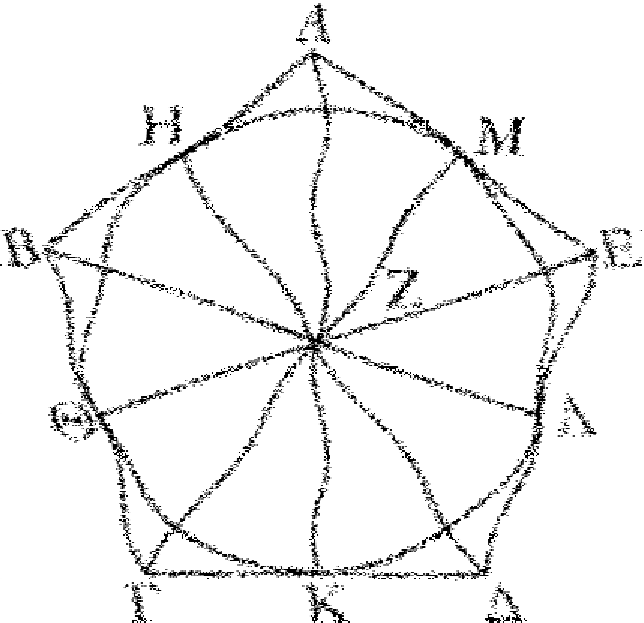
\includegraphics{Book04/front.pdf}}
\newpage

%%%%%%%
% Definitions
%%%%%%%
\pdfbookmark[1]{Definitions}{def4}
\pagestyle{fancy}
\cfoot{\gr{\kern -.7pt }}
\lhead{\large\gr{ΣΤΟΙΘΕΙΩΝ \kern -.7pt {4}.}}
\rhead{\large ELEMENTS BOOK 4}
\begin{Parallel}{}{} 
\ParallelLText{
\begin{center}
\large{\gr{<'Οροι}.}
\end{center}\vspace*{-7pt}

\ggn{1}.~\gr{Σθῆμα εὐθύγραμμον εἰξ σθῆμα εὐθύγραμμον ἐγγράφ\-εσθαι λέγεται, <όταν ἑκάστη τῶν τοῦ ἐγγραφομένου σθήματ\-οξ γωνιῶν
ἑκάστηξ πλευρᾶξ τοῦ, εἰξ <ὸ ἐγγράφεται, <άπτηται.}

\ggn{2}.~\gr{Σθῆμα δὲ ὁμοίωξ περὶ σθῆμα περιγράφεσθαι λέγεται, <όταν ἑκάστη
πλευρὰ τοῦ περιγραφομένου ἑκάστηξ γωνίαξ τοῦ, περὶ <ὸ περιγράφεται,
<άπτηται.}

\ggn{3}.~\gr{Σθῆμα εὐθύγραμμον εἰξ κύκλον ἐγγράφεσθαι λέγεται, <όταν
ἑκάστη γωνία τοῦ ἐγγραφομένου <άπτηται τῆξ τοῦ κύκλου
περιφερείαξ.}

\ggn{4}.~\gr{Σθῆμα δὲ εὐθύγραμμον περὶ κύκλον περιγράφε\-σθαι λέγεται,
<όταν ἑκάστη πλευρὰ τοῦ περιγραφομένου ἐφάπτηται τῆξ τοῦ κύκλου
περιφερείαξ.}

\ggn{5}.~\gr{Κύκλοξ δὲ εἰξ σθῆμα ὁμοίωξ ἐγγράφεσθαι λέγεται, <όταν
ἡ τοῦ κύκλου περιφέρεια ἑκάστηξ πλευρᾶξ τοῦ, εἰξ <ὸ ἐγγράφεται,
<άπτηται.}

\ggn{6}.~\gr{Κύκλοξ δὲ περὶ σθῆμα περιγράφεσθαι λέγεται, <όταν ἡ τοῦ
κύκλου περιφέρεια ἑκάστηξ γωνίαξ τοῦ, περὶ <ὸ περιγράφεται, <άπτηται.}

\ggn{7}.~\gr{Εὐθεῖα εἰξ κύκλον ἐναρμόζεσθαι λέγεται, <όταν τὰ πέρατα
α\kern -.7pt  ὐτῆξ ἐπὶ τῆξ περιφερείαξ >ῆ| τοῦ κύκλου.}}

\ParallelRText{
\begin{center}
{\large Definitions}
\end{center}

1.~A rectilinear figure is said to be inscribed in a(nother) rectilinear figure
when  the respective angles of the inscribed figure touch the respective
sides of the (figure) in which it is inscribed.

2.~And, similarly, a  (rectilinear) figure is said to be circumscribed about a(nother rectilinear) figure when the respective sides of the circumscribed
(figure) touch the respective angles of the (figure) about which it is
circumscribed.

3.~A rectilinear figure is said to be inscribed in a circle when
each angle of the inscribed (figure) touches the circumference of the
circle.

4.~And a rectilinear figure is said to be circumscribed about a circle
when each side of the circumscribed (figure) touches the
circumference of the circle.

5.~And, similarly, a circle is said to be inscribed in a (rectilinear) figure
when the circumference of the circle touches each  side of
the (figure) in which it is inscribed.

6.~And a circle is said to be circumscribed about a rectilinear (figure)
when the circumference of the circle touches each  angle of the
(figure) about which it is circumscribed.

7.~A straight-line is said to be inserted into a circle when its extremities
are on the circumference of the circle.}
\end{Parallel}

%%%%%%
% Prop 4.1
%%%%%%
\pdfbookmark[1]{Proposition 4.1}{pdf4.1}
\begin{Parallel}{}{} 
\ParallelLText{
\begin{center}
{\large \ggn{1}.}
\end{center}\vspace*{-7pt}

\gr{Εἰξ τὸν δοθέντα κύκλον τῆ| δοθείσῃ εὐθείᾳ μ\kern -.7pt  ὴ μείζονι ο>ύσῃ
τῆξ τοῦ κύκλου διαμέτρου >ίσην εὐθεῖαν ἐναρμόσαι.}\\

% Removed epsf size command
\centerline{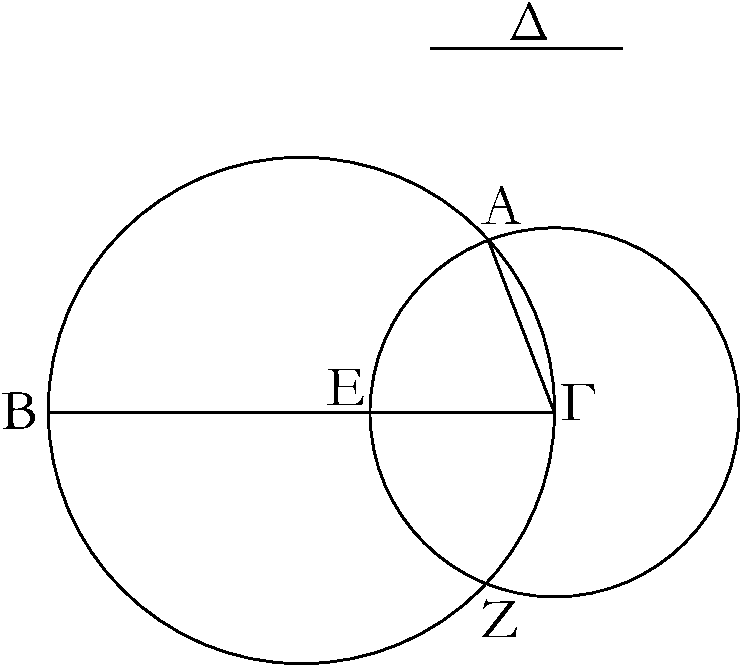
\includegraphics{Book04/fig01g.pdf}}

\gr{>'Εστω ὁ δοθεὶξ κύκλοξ ὁ ΑΒΓ, ἡ δὲ δοθεῖσα εὐθεῖα μ\kern -.7pt  ὴ
μείζων τῆξ τοῦ κύκλου διαμέτρου ἡ Δ. δεῖ δὴ εἰξ τὸν
ΑΒΓ κύκλον τῆ| Δ εὐθείᾳ >ίσην εὐθεῖαν ἐναρμόσαι.}

\gr{>'Ηθθω τοῦ ΑΒΓ κύκλου διάμετροξ ἡ ΒΓ. εἰ μὲν
ο>ῦν >ίση ἐστὶν ἡ ΒΓ τῆ| Δ, γεγονὸξ >ὰν ε>ίη τὸ
ἐπιταθθέν; ἐνήρμοσται γὰρ εἰξ τὸν ΑΒΓ κύκλον τῆ|
Δ εὐθείᾳ >ίση ἡ ΒΓ. εἰ δὲ μείζων ἐστὶν ἡ ΒΓ τῆξ
Δ, κείσθω τῆ| Δ >ίση ἡ ΓΕ, καὶ κέντρῳ τῶ| Γ διαστήματι
δὲ τῶ| ΓΕ κύκλοξ γεγράφθω ὁ ΕΑΖ, καὶ ἐπεζεύθθω
ἡ ΓΑ.}

\gr{Ἐπεὶ ο>ῦν το Γ σημεῖον κέντρον ἐστὶ τοῦ ΕΑΖ κύκλου, >ίση
 ἐστὶν ἡ ΓΑ τῆ| ΓΕ. ἀλλὰ τῆ| Δ ἡ ΓΕ ἐστιν >ίση;
καὶ ἡ Δ >άρα τῆ| ΓΑ ἐστιν >ίση.}

\gr{Εἰξ >άρα τὸν δοθέντα κύκλον τὸν ΑΒΓ τῆ| δοθείσῃ εὐθείᾳ τῆ|
Δ >ίση ἐνήρμοσται ἡ ΓΑ; <όπερ >έδει ποιῆσαι.}}

\ParallelRText{
\begin{center}
{\large Proposition 1}
\end{center}

To insert a straight-line equal to
a given straight-line into a circle, (the latter straight-line) not being greater than the diameter of the circle.

% Removed epsf size command
\centerline{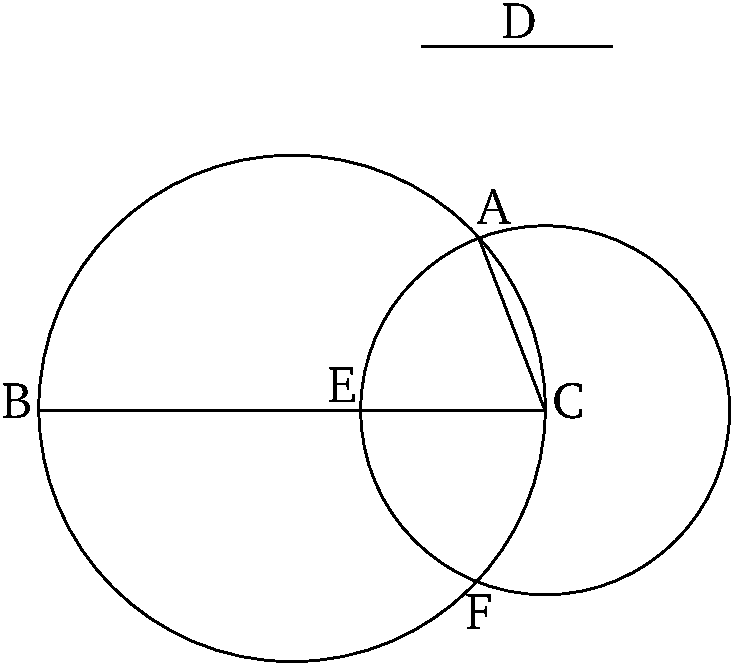
\includegraphics{Book04/fig01e.pdf}}

Let $ABC$ be the given circle, and $D$ the given straight-line (which is) not greater than
the diameter of the circle. So it is required to insert a straight-line, equal to the
straight-line $D$, into the circle $ABC$.

Let a diameter $BC$ of circle $ABC$ be drawn.$^\dag$ Therefore, if
$BC$ is equal to $D$, (then) that (which)  was prescribed has taken place.
For the (straight-line) $BC$, equal to the straight-line $D$, has been inserted into the circle $ABC$.
And if $BC$ is greater than $D$ then let $CE$ be made equal to $D$ [Prop.~1.3], and let the circle $EAF$ be drawn with center $C$ and radius $CE$. And let $CA$ be joined.

Therefore, since the point $C$ is the center of  circle $EAF$, $CA$ is equal to $CE$. But,
$CE$ is equal to $D$. Thus, $D$ is also equal to $CA$.

Thus, $CA$, equal to the given straight-line $D$,  has been inserted into
the given circle $ABC$. (Which is) the very thing it was required to do.}
\end{Parallel}
{\footnotesize \noindent$^\dag$ Presumably, by finding the center of the circle [Prop.~3.1], and then
drawing a line through it.}

%%%%%%
% Prop 4.2
%%%%%%
\pdfbookmark[1]{Proposition 4.2}{pdf4.2}
\begin{Parallel}{}{} 
\ParallelLText{
\begin{center}
{\large \ggn{2}.}
\end{center}\vspace*{-7pt}

\gr{Εἰξ τὸν δοθέντα κύκλον τῶ| δοθέντι τριγώνῳ ἰσογώνιον τρίγωνον
ἐγγράψαι.}

% Removed epsf size command
\centerline{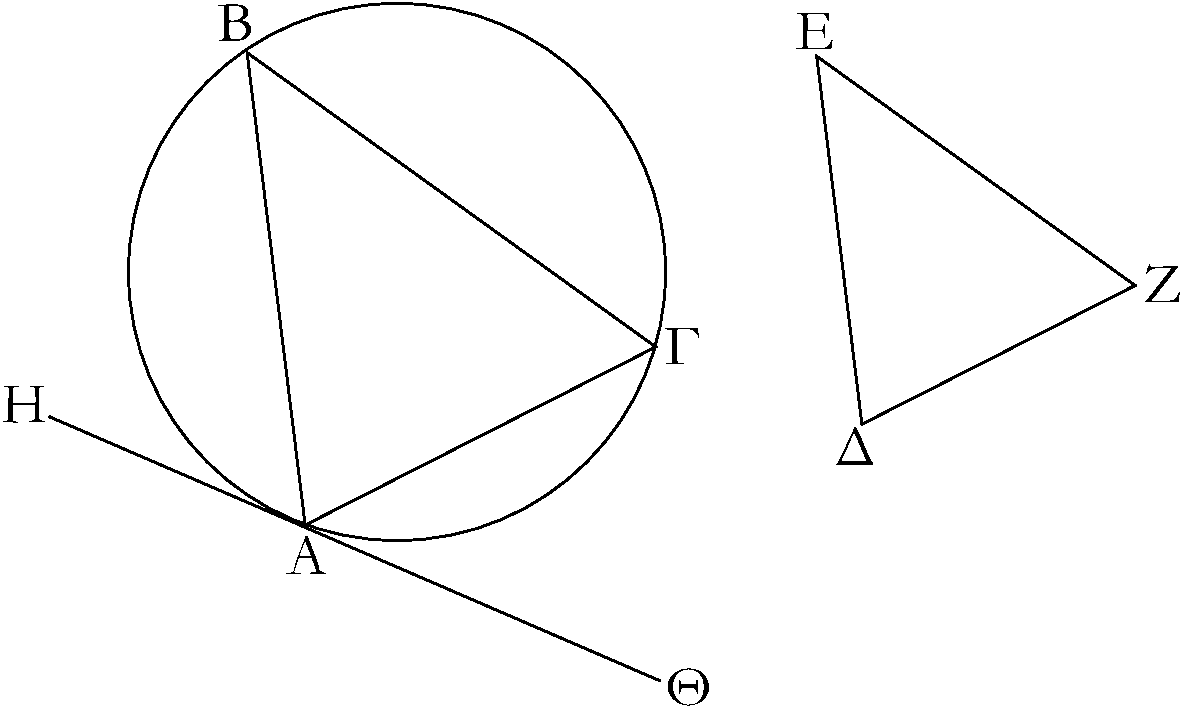
\includegraphics{Book04/fig02g.pdf}}

\gr{>'Εστω ὁ δοθεὶξ κύκλοξ ὁ ΑΒΓ, τὸ δὲ δοθὲν τριγωνον τὸ ΔΕΖ;
δεῖ δὴ εἰξ τὸν ΑΒΓ κύκλον τῶ| ΔΕΖ τριγώνῳ ἰσογώνιον
τρίγωνον ἐγγράψαι.}

\gr{>'Ηθθω τοῦ ΑΒΓ κύκλου ἐφαπτομένη ἡ ΗΘ κατὰ τὸ Α,
καὶ συνεστάτω πρὸξ τῆ| ΑΘ εὐθείᾳ καὶ τῶ| πρὸξ α\kern -.7pt  ὐτῆ| σημείῳ
τῶ| Α τῆ| ὑπὸ ΔΕΖ γωνίᾳ >ίση ἡ ὑπὸ
ΘΑΓ, πρὸξ δὲ τῆ| ΑΗ εὐθείᾳ καὶ τῶ| πρὸξ α\kern -.7pt  ὐτῆ|
σημείῳ τῶ| Α τῆ| ὑπὸ ΔΖΕ [γωνίᾳ] >ίση ἡ ὑπὸ ΗΑΒ, καὶ
ἐπεζεύθθω ἡ ΒΓ.}

\gr{Ἐπεὶ ο>ῦν κύκλου τοῦ ΑΒΓ ἐφάπτεταί τιξ εὐθεῖα ἡ ΑΘ, καὶ
ἀπὸ τῆξ κατὰ τὸ Α ἐπαφῆξ εἰξ τὸν κύκλον διῆκται εὐθεῖα
ἡ ΑΓ, ἡ >άρα ὑπὸ ΘΑΓ >ίση ἐστὶ τῆ| ἐν τῶ| ἐναλλὰχ τοῦ
κύκλου τμ\kern -.7pt  ήματι γωνίᾳ τῆ| ὑπὸ ΑΒΓ. ἀλλ> ἡ ὑπὸ ΘΑΓ τῆ|
ὑπὸ ΔΕΖ ἐστιν >ίση; καὶ ἡ ὑπὸ ΑΒΓ >άρα γωνία τῆ| ὑπὸ
ΔΕΖ ἐστιν >ίση. διὰ τὰ α\kern -.7pt  ὐτὰ δὴ καὶ ἡ ὑπὸ ΑΓΒ τῆ| ὑπὸ
ΔΖΕ ἐστιν >ίση; καὶ λοιπὴ >άρα ἡ ὑπὸ ΒΑΓ λοιπῆ| τῆ| ὑπὸ
ΕΔΖ ἐστιν >ίση [ἰσογώνιον >άρα ἐστὶ τὸ ΑΒΓ τρίγωνον τῶ|
ΔΕΖ τριγώνῳ, καὶ ἐγγέγραπται εἰξ τὸν ΑΒΓ κύκλον].}

\gr{Εἰξ τὸν δοθέντα >άρα κύκλον τῶ| δοθέντι τριγώνῳ
ἰσογώνιον τρίγωνον ἐγγέγραπται; <όπερ >έδει ποιῆσαι.}}

\ParallelRText{
\begin{center}
{\large Proposition 2}
\end{center}

To inscribe a triangle, equiangular with a given triangle, in a given circle.

% Removed epsf size command
\centerline{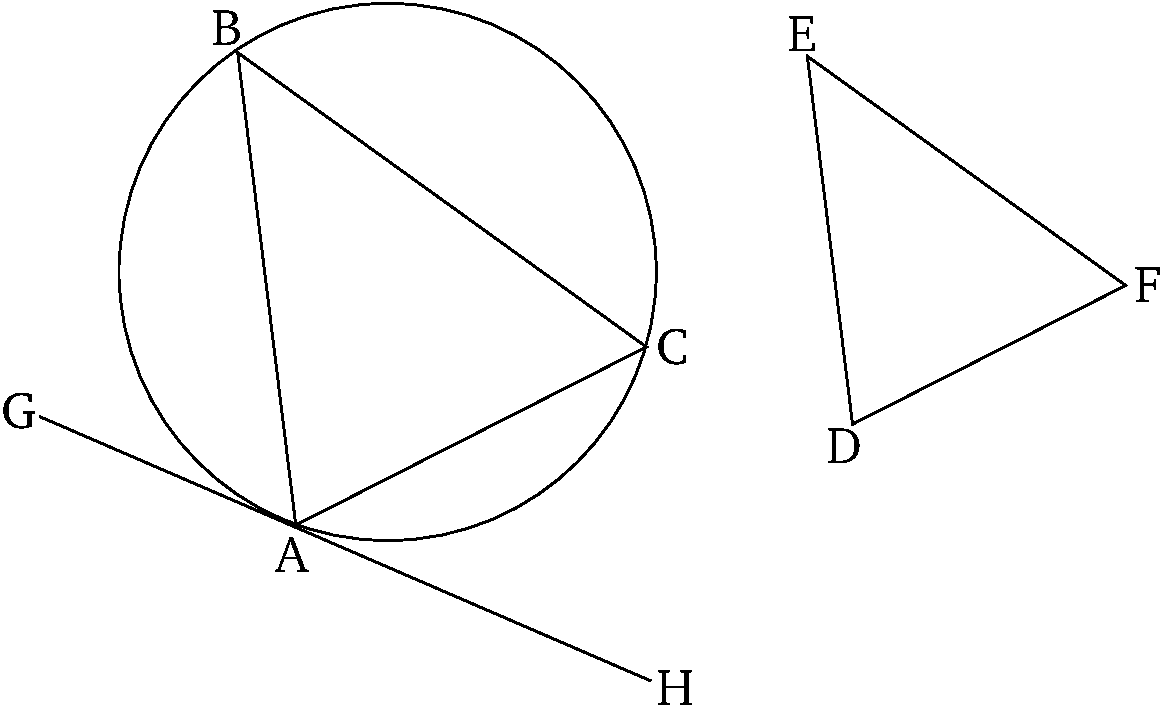
\includegraphics{Book04/fig02e.pdf}}

Let $ABC$ be the given circle, and $DEF$ the given triangle. So it is required
to inscribe a triangle, equiangular with triangle $DEF$, in circle $ABC$.

Let $GH$ be drawn touching circle $ABC$ at $A$.$^\dag$ And let  (angle) $HAC$, equal to angle $DEF$,  be constructed
on the straight-line $AH$ at the point $A$ on it, and (angle) $GAB$, equal to
[angle] $DFE$,  on the straight-line $AG$ at the point $A$ on it
 [Prop.~1.23]. And let $BC$ be joined.
 
 Therefore, since some straight-line $AH$ touches the circle $ABC$, and the
 straight-line $AC$ has been drawn across (the circle) from the point of
 contact $A$, (angle) $HAC$ is thus equal to the angle $ABC$ in the alternate
 segment of the circle [Prop.~3.32]. But, $HAC$ is equal to $DEF$.
 Thus, angle $ABC$ is also equal to $DEF$. So, for the same (reasons),
 $ACB$ is also equal to $DFE$.  Thus, the remaining (angle) $BAC$ is equal
 to the remaining (angle) $EDF$ [Prop.~1.32]. [Thus, triangle
 $ABC$ is equiangular with triangle $DEF$, and has been inscribed in circle
 $ABC$].
 
 Thus, a triangle, equiangular with the given triangle, has been inscribed in
 the given circle. (Which is) the very thing it was required to do.}
\end{Parallel}
{\footnotesize \noindent$^\dag$ See the footnote
to Prop.~3.34.}

%%%%%%
% Prop 4.3
%%%%%%
\pdfbookmark[1]{Proposition 4.3}{pdf4.3}
\begin{Parallel}{}{} 
\ParallelLText{
\begin{center}
{\large \ggn{3}.}
\end{center}\vspace*{-7pt}

\gr{Περὶ τὸν δοθέντα κύκλον τῶ| δοθέντι τριγώνῳ ἰσογώνιον τρίγωνον περιγράψαι.}

% Removed epsf size command
\centerline{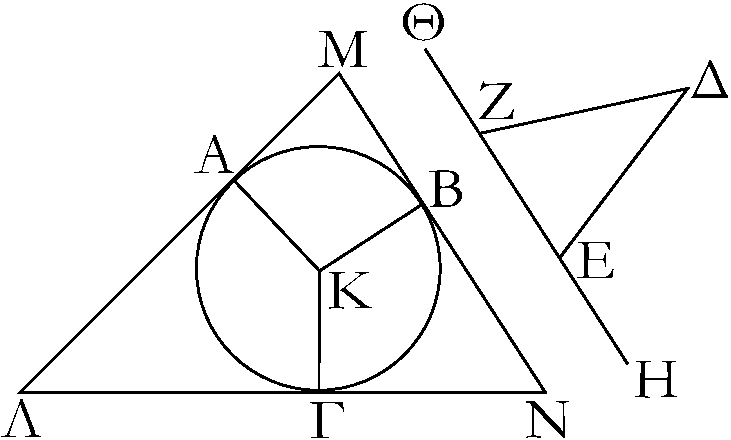
\includegraphics{Book04/fig03g.pdf}}

\gr{>'Εστω ὁ δοθεὶξ κύκλοξ ὁ ΑΒΓ, τὸ δὲ δοθὲν τρίγωνον τὸ ΔΕΖ; δεῖ
δὴ περὶ τὸν ΑΒΓ κύκλον τῶ| ΔΕΖ τριγώνῳ ἰσογώνιον τρίγωνον
περιγράψαι.}

\gr{Ἐκβεβλήσθω ἡ ΕΖ ἐφ> ἑκάτερα τὰ μέρη κατὰ τὰ Η, Θ σημεῖα,
καὶ εἰλήφθω τοῦ ΑΒΓ κύκλου κέντρον τὸ Κ, καὶ διήθθω, ὡξ
>έτυθεν, εὐθεῖα ἡ ΚΒ, καὶ συνεστάτω πρὸξ τῆ| ΚΒ εὐθείᾳ
καὶ τῶ| πρὸξ α\kern -.7pt  ὐτῆ| σημείῳ τῶ| Κ τῆ| μὲν ὑπὸ ΔΕΗ γωνίᾳ
>ίση ἡ ὑπὸ ΒΚΑ, τῆ| δὲ ὑπὸ ΔΖΘ >ίση ἡ ὑπὸ ΒΚΓ, καὶ διὰ
τῶν Α, Β, Γ σημείων >ήθθωσαν ἐφαπτόμεναι τοῦ ΑΒΓ κύκλου
αἱ ΛΑΜ, ΜΒΝ, ΝΓΛ.}

\gr{Καὶ ἐπεὶ ἐφάπτονται τοῦ ΑΒΓ κύκλου αἱ ΛΜ, ΜΝ,
ΝΛ κατὰ τὰ Α, Β, Γ σημεῖα, ἀπὸ δὲ τοῦ Κ κέντρου ἐπὶ
τὰ Α, Β, Γ σημεῖα
ἐπεζευγμέναι εἰσὶν  αἱ ΚΑ, ΚΒ, ΚΓ, ὀρθαὶ >άρα εἰσὶν αἱ
πρὸξ τοῖξ Α, Β, Γ σημείοιξ γωνίαι. καὶ ἐπεὶ τοῦ ΑΜΒΚ τετραπλεύρου αἱ τέσσαρεξ γωνίαι τέτρασιν ὀρθαῖξ >ίσαι εἰσίν, ἐπειδήπερ καὶ
εἰξ δύο τρίγωνα διαιρεῖται τὸ ΑΜΒΚ, καί εἰσιν ὀρθαὶ αἱ ὑπὸ
ΚΑΜ, ΚΒΜ γωνίαι, λοιπαὶ >άρα αἱ ὑπὸ ΑΚΒ, ΑΜΒ δυσὶν ὀρθαῖξ
>ίσαι εἰσίν. εἰσὶ δὲ καὶ αἱ ὑπὸ ΔΕΗ, ΔΕΖ δυσὶν ὀρθαῖξ >ίσαι;
αἱ >άρα ὑπὸ ΑΚΒ, ΑΜΒ ταῖξ ὑπὸ ΔΕΗ, ΔΕΖ >ίσαι εἰσίν,
<ῶν ἡ ὑπὸ ΑΚΒ τῆ| ὑπὸ ΔΕΗ ἐστιν >ίση; λοιπὴ >άρα ἡ ὑπὸ
ΑΜΒ λοιπῆ| τῆ| ὑπὸ ΔΕΖ ἐστιν >ίση.
 ὁμοίωξ δὴ
δειθθήσεται, <ότι καὶ ἡ ὑπὸ ΛΝΒ τῆ| ὑπὸ ΔΖΕ ἐστιν >ίση;
καὶ λοιπὴ >άρα ἡ ὑπὸ ΜΛΝ [λοιπῆ|] τῆ| ὑπὸ ΕΔΖ ἐστιν
>ίση. ἰσογώνιον >άρα ἐστὶ τὸ ΛΜΝ τρίγωνον τῶ| ΔΕΖ
τριγώνῳ; καὶ περιγέγραπται περὶ τὸν ΑΒΓ κύκλον.}

\gr{Περὶ τὸν δοθέντα >άρα κύκλον τῶ| δοθέντι τριγώνῳ ἰσογώνιον
τρίγωνον περιγέγραπται; <όπερ >έδει ποιῆσαι.}}

\ParallelRText{
\begin{center}
{\large Proposition 3}
\end{center}

To circumscribe a triangle, equiangular with a given triangle, about a given
circle.

% Removed epsf size command
\centerline{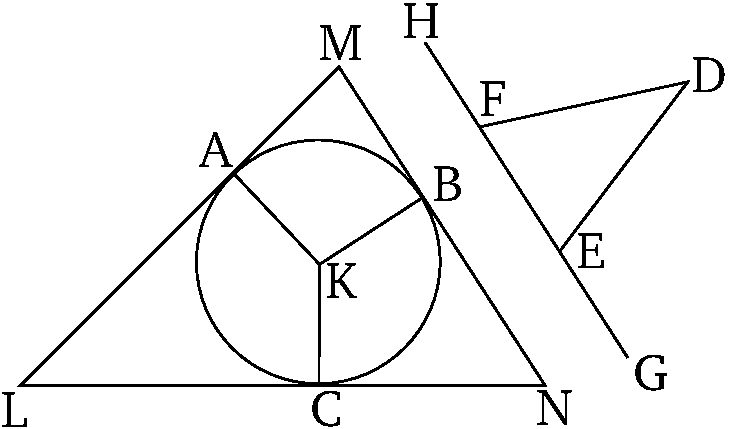
\includegraphics{Book04/fig03e.pdf}}

Let $ABC$ be the given circle, and $DEF$ the given triangle. So it is required
to circumscribe a triangle, equiangular with triangle  $DEF$, about circle $ABC$.

Let $EF$ be produced in each direction to points $G$ and 
$H$. And
let the center $K$ of circle $ABC$ be found [Prop.~3.1].
And let the straight-line $KB$ be drawn, at random,  across ($ABC$).
And let (angle) $BKA$, equal to angle $DEG$, be constructed on the straight-line $KB$ at the point $K$ on it, and (angle) $BKC$, equal to
$DFH$ [Prop.~1.23]. And let the (straight-lines) $LAM$, $MBN$, and $NCL$ be 
drawn through the points $A$, $B$, and $C$ (respectively), touching the circle $ABC$.$^\dag$

And since $LM$, $MN$, and $NL$ touch circle $ABC$ at points $A$, $B$, and $C$
(respectively), and $KA$, $KB$, and $KC$ are joined from the center $K$
to  points $A$, $B$, and $C$ (respectively), the angles at points
$A$, $B$, and $C$ are thus right-angles [Prop.~3.18]. And
since the (sum of the) four angles of quadrilateral $AMBK$ is equal to
four right-angles,
inasmuch as $AMBK$ (can) also (be) divided into two triangles [Prop.~1.32],
and angles $KAM$ and $KBM$ are (both) right-angles, the (sum of the) remaining (angles), $AKB$ and $AMB$, is thus equal to two right-angles. 
And $DEG$ and $DEF$ is also equal to two right-angles [Prop.~1.13].
Thus, $AKB$ and $AMB$ is equal to $DEG$ and $DEF$, of which $AKB$ is
equal to $DEG$. Thus, the remainder $AMB$ is equal to the remainder $DEF$.
So, similarly, it can be shown that $LNB$ is also equal to $DFE$. Thus, the
remaining (angle) $MLN$ is also equal to the [remaining] (angle) $EDF$ [Prop.~1.32]. Thus,
triangle $LMN$ is equiangular with triangle $DEF$. And it has been drawn around
circle $ABC$.

Thus,  a triangle, equiangular with  the given triangle, has been circumscribed about the given
circle. (Which is) the very thing it was required to do.}
\end{Parallel}
{\footnotesize \noindent$^\dag$ See the footnote
to Prop.~3.34.}

%%%%%%
% Prop 4.4
%%%%%%
\pdfbookmark[1]{Proposition 4.4}{pdf4.4}
\begin{Parallel}{}{} 
\ParallelLText{
\begin{center}
{\large \ggn{4}.}
\end{center}\vspace*{-7pt}

\gr{Εἰξ τὸ δοθὲν  τρίγωνον κύκλον ἐγγράψαι.}

% Removed epsf size command
\centerline{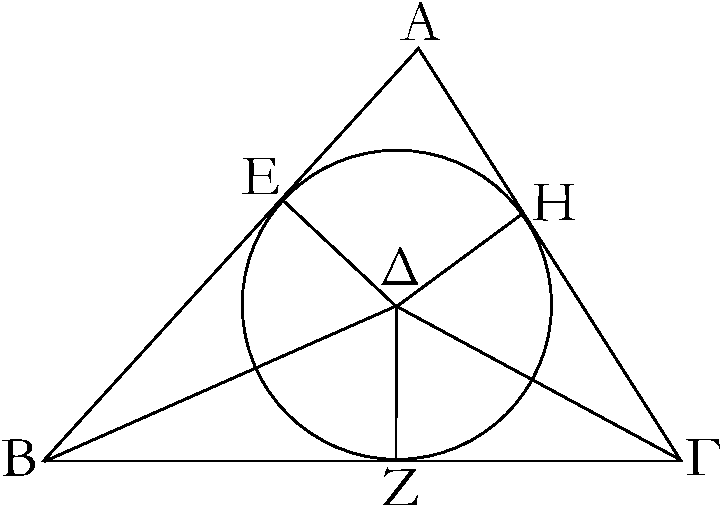
\includegraphics{Book04/fig04g.pdf}}

\gr{>'Εστω τὸ δοθὲν τρίγωνον τὸ ΑΒΓ; δεῖ δὴ εἰξ τὸ ΑΒΓ τρίγωνον κύκλον ἐγγράψαι.}

\gr{Τετμ\kern -.7pt  ήσθωσαν αἱ ὑπὸ ΑΒΓ, ΑΓΒ γωνίαι δίθα ταῖξ ΒΔ, ΓΔ εὐθείαιξ,
καὶ συμβαλλέτωσαν ἀλλήλαιξ κατὰ τὸ Δ σημεῖον, καὶ >ήθθωσαν ἀπὸ
τοῦ Δ ἐπὶ τὰξ ΑΒ, ΒΓ, ΓΑ 	εὐθείαξ κάθετοι αἱ ΔΕ, ΔΖ, ΔΗ.}

\gr{Καὶ ἐπεὶ >ίση ἐστὶν ἡ ὑπὸ ΑΒΔ γωνία τῆ| ὑπὸ ΓΒΔ, ἐστὶ
δὲ καὶ ὀρθὴ ἡ ὑπὸ ΒΕΔ ὀρθῆ| τῆ| ὑπὸ ΒΖΔ >ίση, δύο
δὴ τρίγωνά ἐστι τὰ ΕΒΔ, ΖΒΔ τὰξ δύο γωνίαξ ταῖξ δυσὶ γωνίαιξ
>ίσαξ >έθοντα καὶ μίαν πλευρὰν μιᾶ| πλευρᾶ| >ίσην τὴν ὑποτείνουσαν
ὑπὸ μίαν
τῶν >ίσων γωνιῶν κοινὴν α\kern -.7pt  ὐτῶν τὴν
ΒΔ; καὶ τὰξ λοιπὰξ >άρα πλευρὰξ ταῖξ λοιπαῖξ πλευραῖξ >ίσαξ
<έχουσιν; >ίση >άρα ἡ ΔΕ τῆ| ΔΖ. διὰ τὰ α\kern -.7pt  ὐτὰ δὴ καὶ ἡ
ΔΗ τῆ| ΔΖ ἐστιν >ίση. αἱ τρεῖξ >άρα εὐθεῖαι αἱ ΔΕ, ΔΖ, ΔΗ
>ίσαι ἀλλήλαιξ εἰσίν; ὁ >άρα κέντρῶ| τῶ| Δ καὶ διαστήματι
ἑνὶ τῶν Ε, Ζ, Η κύκλοξ γραφόμενοξ <ήχει καὶ διὰ τῶν λοιπῶν
σημείων καὶ ἐφάψεται τῶν ΑΒ, ΒΓ, ΓΑ εὐθειῶν διὰ τὸ ὀρθὰξ ε>ῖναι τὰξ πρὸξ τοῖξ Ε, Ζ, Η σημείοιξ γωνίαξ. εἰ γὰρ τεμεῖ
α\kern -.5pt  ὐτάξ, >έσται ἡ τῆ| διαμέτρῳ τοῦ κύκλου πρὸξ ὀρθὰξ
ἀπ> >άκραξ ἀγομένη ἐντὸξ πίπτουσα τοῦ κύκλου; <όπερ
>άτοπον ἐδείθθη; οὐκ >άρα ὁ κέντρῳ τῶ| Δ διαστήματι
δὲ ἑνὶ τῶν Ε, Ζ, Η γραφόμενοξ κύκλοξ τεμεῖ τὰξ ΑΒ, ΒΓ, ΓΑ εὐθείαξ; ἐφάψεται >άρα α\kern -.3pt  ὐτῶν, καὶ >έσται ὁ 
κύκλοξ ἐγγεγραμμένοξ εἰξ τὸ ΑΒΓ τρίγωνον. 
ἐγγεγράφθω ὡξ ὁ ΖΗΕ.}

\gr{Εἰξ >άρα τὸ δοθὲν τρίγωνον τὸ ΑΒΓ κύκλοξ
ἐγγέγρ\-απται ὁ ΕΖΗ; <όπερ >έδει ποιῆσαι.}}

\ParallelRText{
\begin{center}
{\large Proposition 4}
\end{center}

To inscribe a circle in a given triangle.

% Removed epsf size command
\centerline{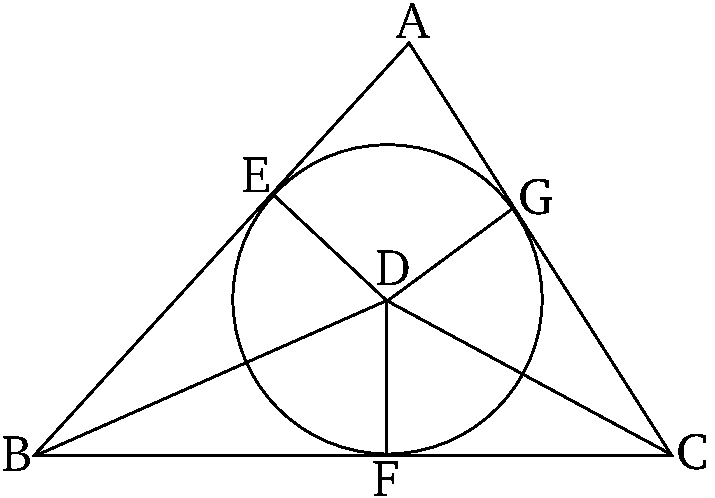
\includegraphics{Book04/fig04e.pdf}}

Let $ABC$ be the given triangle. So it is required to inscribe
a circle in triangle $ABC$.

Let the angles $ABC$ and $ACB$ be cut in half by the
straight-lines $BD$ and $CD$ (respectively) [Prop.~1.9], and let them meet one another
at point $D$, and let $DE$, $DF$, and $DG$ be drawn from
point $D$, perpendicular to the straight-lines $AB$, $BC$, and $CA$ (respectively) [Prop.~1.12].

And since angle $ABD$ is equal to $CBD$, and the right-angle
$BED$ is also equal to the right-angle $BFD$, $EBD$ and $FBD$ are thus two triangles
having two angles equal to two angles, and one side equal to one side---the
(one) subtending one of the equal angles (which is) common to the (triangles)---(namely), $BD$. Thus, they will also have the 
remaining sides equal to the (corresponding) remaining sides [Prop.~1.26]. Thus, $DE$ (is)
equal to $DF$. So, for the same (reasons), $DG$ is also equal
to $DF$. Thus, the three straight-lines $DE$, $DF$, and $DG$ are equal to one another.
Thus, the circle drawn with center $D$, and radius one of $E$, $F$, or $G$,$^\dag$ will also
go through the remaining points, and will  touch the straight-lines $AB$, $BC$, and $CA$, on account of the angles at $E$, $F$, and $G$ being right-angles. For if it cuts (one of) them then it will be a (straight-line)
drawn at right-angles to a diameter of the circle, from its extremity, falling inside
the circle. The very thing was shown (to be) absurd [Prop.~3.16].
Thus, the circle drawn with center $D$, and radius one of $E$, $F$, or $G$,
does not cut the straight-lines $AB$, $BC$, and $CA$. Thus, it will
touch them, and will be the circle inscribed  in triangle $ABC$.
Let it be (so) inscribed, like $FGE$ (in the figure).

Thus, the circle $EFG$ has been inscribed in the given triangle $ABC$.
(Which is) the very thing it was required to do.}
\end{Parallel}
{\footnotesize \noindent$^\dag$ Here, and in the following propositions, it
is understood that the radius is actually one of $DE$, $DF$, or $DG$.}

%%%%%%
% Prop 4.5
%%%%%%
\pdfbookmark[1]{Proposition 4.5}{pdf4.5}
\begin{Parallel}{}{} 
\ParallelLText{
\begin{center}
{\large \ggn{5}.}
\end{center}\vspace*{-7pt}

\gr{Περὶ τὸ δοθὲν τρίγωνον κύκλον περιγράψαι.}

% Removed epsf size command
\centerline{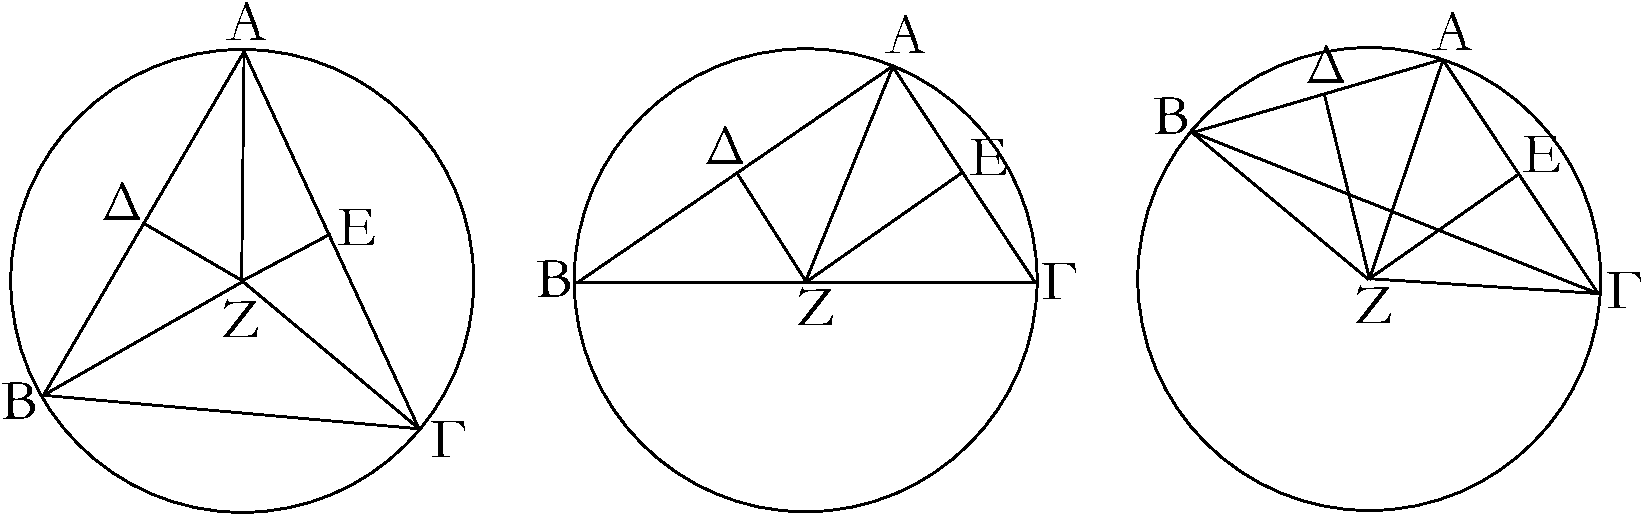
\includegraphics{Book04/fig05g.pdf}}

\gr{>'Εστω τὸ δοθὲν τρίγωνον τὸ ΑΒΓ; δεῖ δὲ περὶ τὸ δοθὲν τρίγωνον
τὸ ΑΒΓ κύκλον περιγράψαι.}

\gr{Τετμ\kern -.7pt  ήσθωσαν αἱ ΑΒ, ΑΓ εὐθεῖαι δίθα κατὰ τὰ Δ, Ε σημεῖα, καὶ
ἀπὸ τῶν Δ, Ε σημείων ταῖξ ΑΒ, ΑΓ πρὸξ ὀρθὰξ >ήθθωσαν
αἱ ΔΖ, ΕΖ; συμπεσοῦνται δὴ >ήτοι ἐντὸξ τοῦ ΑΒΓ τριγώνου
>ὴ ἐπὶ τῆξ ΒΓ εὐθείαξ >ὴ ἐκτὸξ τῆξ ΒΓ.}

\gr{Συμπιπτέτωσαν πρότερον ἐντὸξ κατὰ τὸ Ζ, καὶ ἐπεζεύθθ\-ωσαν
αἱ ΖΒ, ΖΓ, ΖΑ. καὶ ἐπεὶ >ίση ἐστὶν ἡ ΑΔ τῆ| ΔΒ, κοινὴ
δὲ καὶ πρὸξ ὀρθὰξ ἡ ΔΖ, βάσιξ >άρα ἡ ΑΖ βάσει τῆ| ΖΒ
ἐστιν >ίση. ὁμοίωξ δὴ δείχομεν, <ότι καὶ ἡ ΓΖ τῆ| ΑΖ ἐστιν
>ίση; <ώστε καὶ ἡ ΖΒ τῆ| ΖΓ ἐστιν >ίση; αἱ τρεῖξ
>άρα αἱ ΖΑ, ΖΒ, ΖΓ >ίσαι  ἀλλήλαιξ εἰσίν. ὁ >άρα κέντρῳ
τῶ| Ζ διαστήματι δὲ ἑνὶ τῶν Α, Β, Γ κύκλοξ γραφόμενοξ <ήχει
καὶ διὰ τῶν λοιπῶν σημείων, καὶ >έσται περιγεγραμμένοξ
ὁ κύκλοξ περὶ τὸ ΑΒΓ τρίγωνον. περιγεγράφθω ὡξ ὁ ΑΒΓ.}

\gr{Ἀλλὰ δὴ αἱ ΔΖ, ΕΖ συμπιπτέτωσαν ἐπὶ τῆξ ΒΓ εὐθείαξ
κατὰ τὸ Ζ, ὡξ >έθει ἐπὶ τῆξ δευτέραξ καταγραφῆξ, καὶ
ἐπεζεύθθω ἡ ΑΖ. ὁμοίωξ δὴ δείχομεν, <ότι τὸ Ζ σημεῖον
κέντρον ἐστὶ τοῦ περὶ τὸ ΑΒΓ τρίγωνον περιγραφομένου κύκλου.}

\gr{Ἀλλὰ δὴ αἱ ΔΖ, ΕΖ συμπιπτέτωσαν ἐκτὸξ τοῦ ΑΒΓ τριγώνου κατὰ
τὸ Ζ πάλιν, ὡξ >έθει ἐπὶ τῆξ τρίτηξ καταγραφῆξ, καί 
ἐπεζεύθθωσαν αἱ ΑΖ, ΒΖ, ΓΖ. καὶ ἐπεὶ πάλιν >ίση ἐστὶν ἡ
ΑΔ τῆ| ΔΒ, κοινὴ δὲ καὶ πρὸξ ὀρθὰξ ἡ ΔΖ, βάσιξ >άρα
ἡ ΑΖ βάσει τῆ| ΒΖ ἐστιν >ίση. ὁμοίωξ δὴ δείχομεν, <ότι
καὶ ἡ ΓΖ τῆ| ΑΖ ἐστιν >ίση; <ώστε καὶ ἡ ΒΖ τῆ| ΖΓ ἐστιν
>ίση; ὁ >άρα [πάλιν] κέντρῳ τῶ| Ζ διαστήματι δὲ ἑνὶ τῶν
ΖΑ, ΖΒ, ΖΓ κύκλοξ γραφόμενοξ <ήχει καὶ διὰ τῶν λοιπῶν σημείων,
καὶ >έσται περιγεγραμμένοξ περὶ τὸ ΑΒΓ τρίγωνον.}

\gr{Περὶ τὸ δοθὲν >άρα τρίγωνον κύκλοξ περιγέγραπται; <όπερ >έδει ποιῆσαι.}}

\ParallelRText{
\begin{center}
{\large Proposition 5}
\end{center}

To circumscribe a circle about a given  triangle.

% Removed epsf size command
\centerline{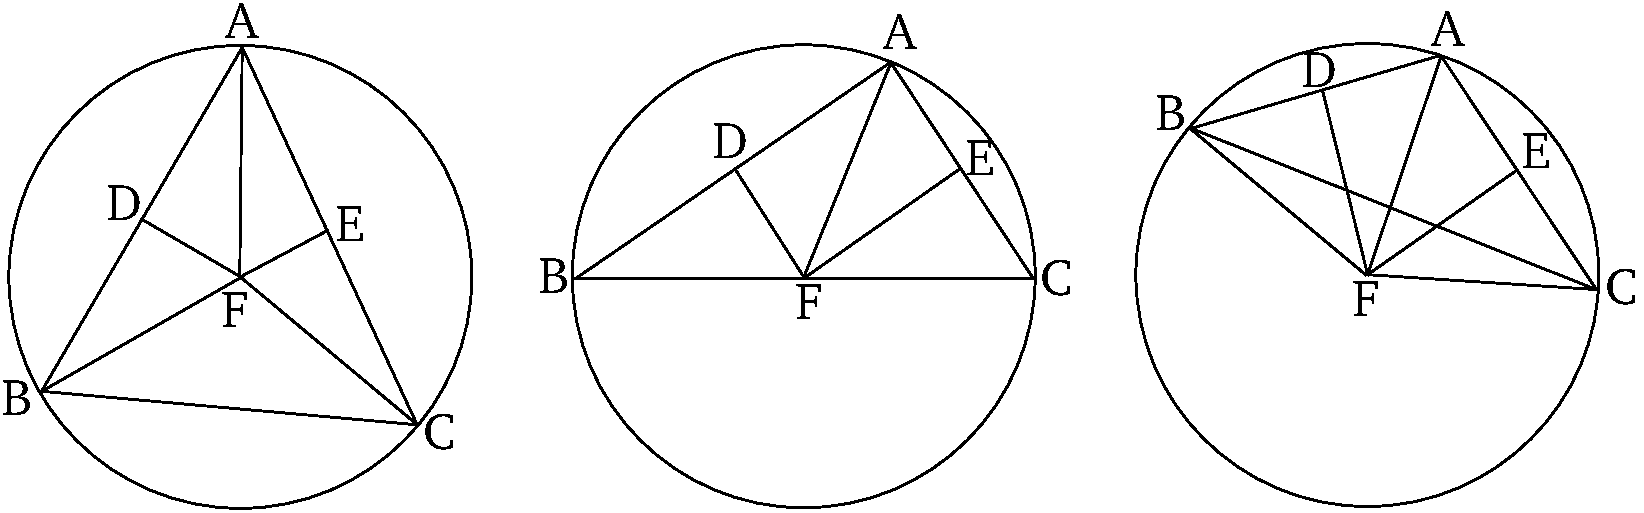
\includegraphics{Book04/fig05e.pdf}}

Let $ABC$ be the given triangle. So it is required to circumscribe
a circle about the given triangle $ABC$.

Let the straight-lines $AB$ and $AC$ be cut in half at points $D$ and $E$ (respectively) [Prop.~1.10]. And let $DF$ and $EF$ be drawn from 
points $D$ and $E$, at right-angles to $AB$ and $AC$ (respectively) [Prop.~1.11].
So  ($DF$ and $EF$) will surely either meet inside triangle $ABC$, on the straight-line
$BC$, or beyond $BC$.

Let them, first of all, meet inside (triangle $ABC$) at (point) $F$, and let $FB$, 
$FC$, and $FA$ be joined. And since $AD$ is equal to $DB$, and $DF$ is
common and at right-angles, the base $AF$ is thus equal to the base $FB$
[Prop.~1.4]. So, similarly, we can show that $CF$ is also equal to
$AF$. So that $FB$ is also equal to $FC$. Thus, the three (straight-lines)
$FA$, $FB$, and $FC$ are equal to one another. Thus, the circle drawn with
center $F$, and radius one of $A$, $B$, or $C$, will also go through the remaining points.
And the circle will be circumscribed about triangle $ABC$. Let it
be (so) circumscribed, like $ABC$ (in the first diagram from the left).

And so, let $DF$ and $EF$ meet on the straight-line $BC$ at (point) $F$, like
in the second diagram (from the left). And let $AF$ be joined.
So, similarly, we can show that point $F$ is the center of the circle circumscribed about triangle $ABC$.

And so, let $DF$ and $EF$ meet outside triangle $ABC$, again at (point) $F$, like
in the third diagram (from the left). And let $AF$, $BF$, and $CF$ be joined.
And, again, since $AD$ is equal to $DB$, and $DF$ is common and at right-angles,
the base $AF$ is thus equal to the base $BF$ [Prop.~1.4]. So, similarly,
we can show that $CF$ is also equal to $AF$. So that $BF$ is also equal to $FC$.
Thus, [again] the circle drawn with center $F$, and radius one of $FA$, $FB$, and
$FC$, will also go through the remaining points. And it will be circumscribed
about triangle $ABC$.

Thus, a circle has been circumscribed about the given triangle. (Which is)
the very thing it was required to do.}
\end{Parallel}

%%%%%%
% Prop 4.6
%%%%%%
\pdfbookmark[1]{Proposition 4.6}{pdf4.6}
\begin{Parallel}{}{} 
\ParallelLText{
\begin{center}
{\large \ggn{6}.}
\end{center}\vspace*{-7pt}

\gr{Εἰξ τὸν δοθέντα κύκλον τετράγωνον ἐγγράψαι.}

\gr{>'Εστω ἡ δοθεὶξ κύκλοξ ὁ ΑΒΓΔ; δεῖ δὴ εἰξ τὸν ΑΒΓΔ κύκλον
τετράγωνον ἐγγράψαι.}

\gr{>'Ηθθωσαν τοῦ ΑΒΓΔ κύκλου δύο διάμετροι πρὸξ ὀρθὰξ ἀλλήλαιξ
αἱ ΑΓ, ΒΔ, καὶ ἐπεζεύθθωσαν αἱ ΑΒ, ΒΓ, ΓΔ, ΔΑ.}\\

% Removed epsf size command
\centerline{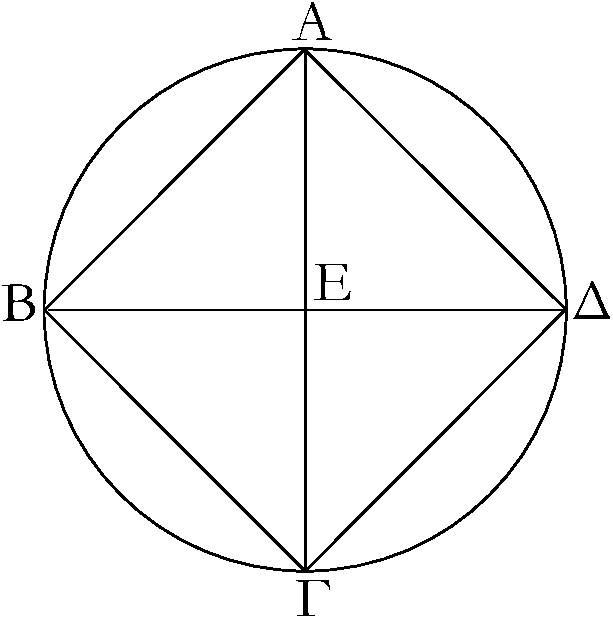
\includegraphics{Book04/fig06g.pdf}}

\gr{Καὶ ἐπεὶ >ίση ἐστὶν ἡ ΒΕ τῆ| ΕΔ; κέντρον γὰρ τὸ Ε; κοινὴ
δὲ καὶ πρὸξ ὀρθὰξ ἡ ΕΑ, βάσιξ >άρα ἡ ΑΒ βάσει τῆ| ΑΔ >ίση
ἐστίν. διὰ τὰ α\kern -.7pt  ὐτὰ δὴ καὶ ἑκατέρα τῶν ΒΓ, ΓΔ ἑκατέρᾳ  τῶν ΑΒ, 
ΑΔ >ίση ἐστίν; ἰσόπλευρον >άρα ἐστὶ τὸ ΑΒΓΔ τετράπλευρον. λέγω
δή, <ότι καὶ ὀρθογώνιον. ἐπεὶ γὰρ ἡ ΒΔ εὐθεῖα  διάμετρόξ ἐστι
τοῦ ΑΒΓΔ κύκλου, ἡμικύκλιον >άρα ἐστὶ τὸ ΒΑΔ; ὀρθὴ >άρα
ἡ ὑπὸ ΒΑΔ γωνία. διὰ τὰ α\kern -.7pt  ὐτὰ δὴ καὶ ἑκάστη τῶν ὑπὸ ΑΒΓ, ΒΓΔ, ΓΔΑ ὀρθή ἐστιν; ὀρθογώνιον >άρα ἐστὶ τὸ ΑΒΓΔ τετράπλευρον.
ἐδείθθη δὲ καὶ ἰσόπλευρον; τετράγωνον >άρα ἐστίν. καὶ
ἐγγέγραπται εἰξ τὸν ΑΒΓΔ κύκλον.}

\gr{Εἰξ >άρα τὸν δοθέντα κύκλον τετράγωνον ἐγγέγραπται τὸ ΑΒΓΔ; <όπερ
>έδει ποιῆσαι.}}

\ParallelRText{
\begin{center}
{\large Proposition 6}
\end{center}

To inscribe a square in a given circle.

Let $ABCD$ be the given circle. So it is required to inscribe a square in circle
$ABCD$.

Let two diameters  of circle $ABCD$,  $AC$ and $BD$, be drawn at right-angles to one another.$^\dag$ And let $AB$, $BC$, $CD$, and $DA$ be joined.

% Removed epsf size command
\centerline{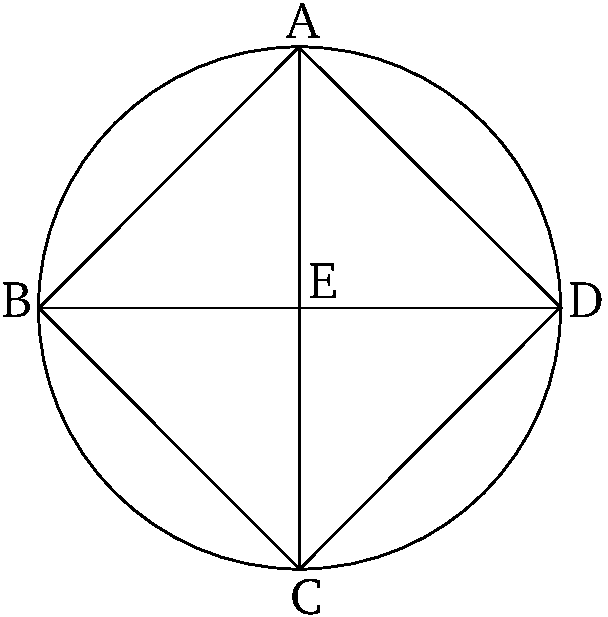
\includegraphics{Book04/fig06e.pdf}}

And since $BE$ is equal to $ED$, for $E$ (is) the center (of the circle), and $EA$
is common and at right-angles, the base $AB$ is thus equal to the base $AD$ [Prop.~1.4]. So, for the same (reasons), each of $BC$ and $CD$ is equal
to each of $AB$ and $AD$. Thus, the quadrilateral $ABCD$ is equilateral. So I say
that (it is) also right-angled. For since the straight-line $BD$ is a diameter
of circle $ABCD$, $BAD$ is thus a semi-circle. Thus, angle $BAD$ (is) a right-angle
[Prop.~3.31]. So, for the same (reasons), (angles)
$ABC$, $BCD$, and $CDA$ are also each right-angles. Thus, the quadrilateral $ABCD$
is right-angled. And it was also shown (to be) equilateral. Thus, it is a square [Def.~1.22]. And it has been inscribed in circle
$ABCD$.

Thus, the square $ABCD$ has been inscribed in the given circle. (Which is)
the very thing it was required to do.}
\end{Parallel}
{\footnotesize \noindent$^\dag$ Presumably, by finding the center of the circle [Prop.~3.1], 
drawing a line through it, and then drawing a second line through it, at right-angles to the first [Prop.~1.11].} 

%%%%%%
% Prop 4.7
%%%%%%
\pdfbookmark[1]{Proposition 4.7}{pdf4.7}
\begin{Parallel}{}{} 
\ParallelLText{
\begin{center}
{\large \ggn{7}.}
\end{center}\vspace*{-7pt}

\gr{Περὶ τὸν δοθέντα κύκλον τετράγωνον περιγράψαι.}

\gr{>'Εστω ὁ δοθεὶξ κύκλοξ ὁ ΑΒΓΔ; δεῖ δὴ περὶ τὸν ΑΒΓΔ κύκλον
τετράγωνον περιγράψαι.}

\gr{>'Ηθθωσαν τοῦ ΑΒΓΔ κύκλου δύο διάμετροι πρὸξ ὀρθὰξ ἀλλήλαιξ
αἱ ΑΓ, ΒΔ, καὶ διὰ τῶν Α, Β, Γ, Δ σημείων >ήθθωσαν ἐφαπτόμεναι
τοῦ ΑΒΓΔ κύκλου αἱ ΖΗ, ΗΘ, ΘΚ, ΚΖ.}

\gr{Ἐπεὶ ο>ῦν ἐφάπτεται ἡ ΖΗ τοῦ ΑΒΓΔ κύκλου, ἀπὸ δὲ τοῦ Ε κέντρου ἐπὶ τὴν κατὰ τὸ Α ἐπαφὴν ἐπέζευκται ἡ ΕΑ, αἱ
>άρα πρὸξ τῶ| Α γωνίαι ὀρθαί εἰσιν. διὰ τὰ α\kern -.7pt  ὐτὰ δὴ καὶ αἱ
πρὸξ τοῖξ Β, Γ, Δ σημείοιξ γωνίαι ὀρθαί εἰσιν. καὶ ἐπεὶ
ὀρθή ἐστιν ἡ ὑπὸ ΑΕΒ γωνία, ἐστὶ δὲ ὀρθὴ καὶ ἡ ὑπὸ
ΕΒΗ, παράλληλοξ >άρα ἐστὶν ἡ ΗΘ τῆ| ΑΓ. διὰ τὰ α\kern -.7pt  ὐτὰ
δὴ καὶ ἡ ΑΓ τῆ| ΖΚ ἐστι παράλληλοξ. <ώστε καὶ ἡ ΗΘ τῆ|
ΖΚ ἐστι παράλληλοξ. ὁμοίωξ δὴ δείχομεν, <ότι καὶ ἑκατέρα
τῶν ΗΖ, ΘΚ τῆ| ΒΕΔ ἐστι παράλληλοξ. παραλληλόγραμμα >άρα ἐστὶ
τὰ ΗΚ, ΗΓ, ΑΚ, ΖΒ, ΒΚ; >ίση >άρα ἐστὶν ἡ μὲν ΗΖ τῆ| ΘΚ,
ἡ δὲ ΗΘ τῆ| ΖΚ. καὶ ἐπεὶ >ίση ἐστὶν ἡ ΑΓ τῆ| ΒΔ, ἀλλὰ
καὶ ἡ μὲν ΑΓ ἑκατέρᾳ τῶν ΗΘ, ΖΚ, ἡ δὲ ΒΔ ἑκατέρᾳ
τῶν ΗΖ, ΘΚ ἐστιν >ίση [καὶ ἑκατέρα >άρα τῶν ΗΘ, ΖΚ ἑκατέρᾳ
τῶν ΗΖ, ΘΚ ἐστιν >ίση], ἰσόπλευρον >άρα ἐστὶ τὸ ΖΗΘΚ
τετράπλευρον. λέγω δή, <ότι
καὶ ὀρθογώνιον. ἐπεὶ γὰρ παραλληλόγραμμόν ἐστι τὸ ΗΒΕΑ,
καί ἐστιν ὀρθὴ ἡ ὑπὸ ΑΕΒ, ὀρθὴ >άρα καὶ ἡ ὑπὸ ΑΗΒ. ὁμοίωξ
δὴ δείχομεν, <ότι καὶ αἱ πρὸξ τοῖξ Θ, Κ, Ζ γωνίαι ὀρθαί
εἰσιν. ὀρθογώνιον >άρα ἐστὶ τὸ ΖΗΘΚ. ἐδείθθη δὲ καὶ ἰσόπλευρον;
τετράγωνον >άρα ἐστίν. καὶ περιγέγραπται περὶ τὸν ΑΒΓΔ κύκλον.}

% Removed epsf size command
\centerline{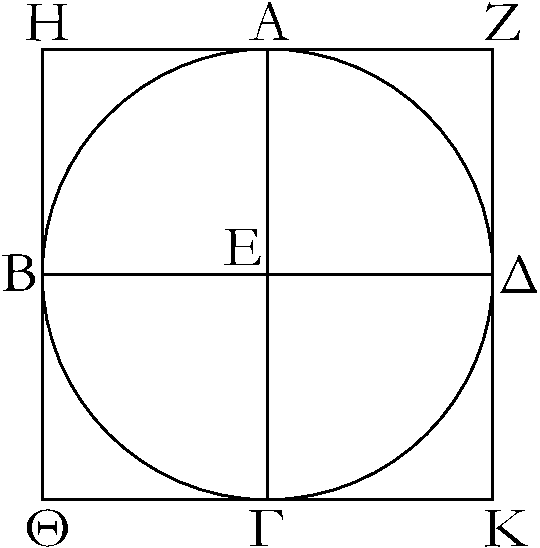
\includegraphics{Book04/fig07g.pdf}}

\gr{Περὶ τὸν δοθέντα >άρα κύκλον τετράγωνον περιγέγραπται;
<όπερ >έδει ποιῆσαι.}}

\ParallelRText{
\begin{center}
{\large Proposition 7}
\end{center}

To circumscribe a square about a given circle.

Let $ABCD$ be the given circle. So it is required to circumscribe a square
about circle $ABCD$.
Let two diameters of circle $ABCD$,  $AC$ and $BD$,  be drawn at right-angles to one another.$^\dag$
And let $FG$, $GH$, $HK$, and $KF$ be drawn through points $A$, $B$, $C$, and
$D$ (respectively), touching circle $ABCD$.$^\ddag$

Therefore, since $FG$ touches circle $ABCD$, and $EA$ has been joined from the
center $E$ to the point of contact $A$, the angles at $A$ are thus  right-angles  
[Prop.~3.18]. So, for the same (reasons), the angles at points $B$, $C$, and $D$ are also
right-angles. And since angle $AEB$ is a right-angle, and $EBG$ is also a right-angle, $GH$ is thus parallel to $AC$ [Prop.~1.29]. So, for the same
(reasons), $AC$ is also parallel to $FK$. So that $GH$ is also parallel to
$FK$ [Prop.~1.30]. So, similarly, we can show that $GF$ and $HK$ are each parallel to
$BED$. Thus, $GK$, $GC$, $AK$, $FB$, and $BK$ are (all) parallelograms. Thus, 
$GF$ is equal to $HK$, and $GH$ to $FK$ [Prop.~1.34]. And since
$AC$ is equal to $BD$, but $AC$ (is) also (equal) to each of $GH$ and $FK$,
and $BD$ is equal to each of $GF$ and $HK$ [Prop.~1.34] [and each of $GH$ and $FK$ is thus equal to each of $GF$ and $HK$], the quadrilateral $FGHK$ is
thus equilateral.  So I say that (it is) also right-angled. For since $GBEA$
is a parallelogram, and $AEB$ is a right-angle, $AGB$ is thus also a right-angle [Prop.~1.34]. So, similarly, we can show that the angles at $H$, $K$, and
$F$ are also right-angles. Thus, $FGHK$ is right-angled. And it was also shown
(to be) equilateral. Thus,  it is a square [Def.~1.22].
And it has been circumscribed about circle $ABCD$.

% Removed epsf size command
\centerline{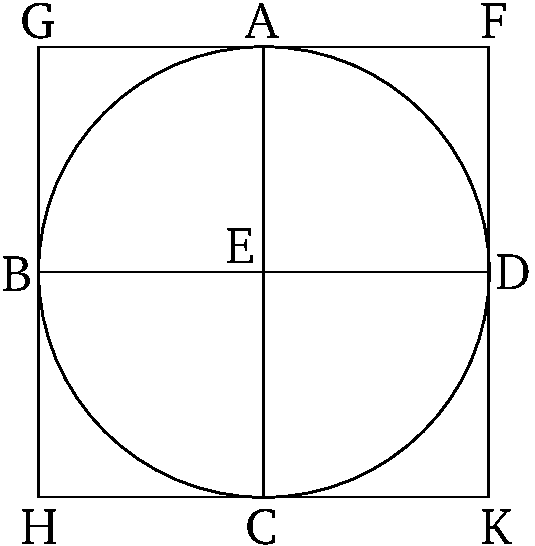
\includegraphics{Book04/fig07e.pdf}}

Thus, a square has been circumscribed about the given circle. (Which is)
the very thing it was required to do.}
\end{Parallel}
{\footnotesize \noindent$^\dag$ See the footnote to the previous
 proposition.\\
 $^\ddag$ See the footnote
to Prop.~3.34.}

%%%%%%
% Prop 4.8
%%%%%%
\pdfbookmark[1]{Proposition 4.8}{pdf4.8}
\begin{Parallel}{}{} 
\ParallelLText{
\begin{center}
{\large \ggn{8}.}
\end{center}\vspace*{-7pt}

\gr{Εἰξ τὸ δοθὲν τετράγωνον κύκλον ἐγγράψαι.}

\gr{>'Εστω τὸ δοθὲν τετράγωνον τὸ ΑΒΓΔ; δεῖ δὴ εἰξ τὸ ΑΒΓΔ
τετράγωνον κύκλον ἐγγράψαι.}

% Removed epsf size command
\centerline{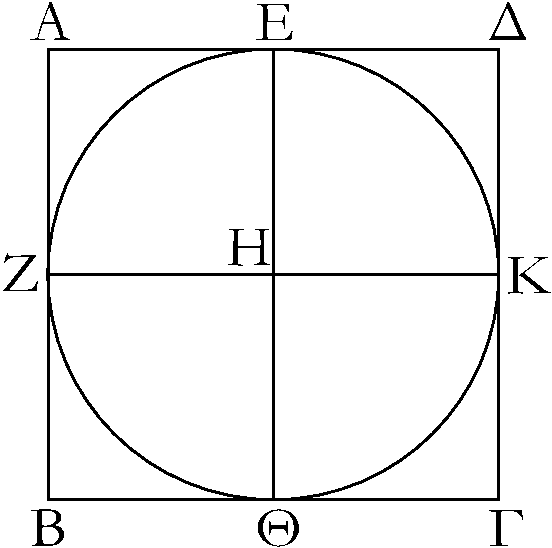
\includegraphics{Book04/fig08g.pdf}}

\gr{Τετμ\kern -.7pt  ήσθω ἑκατέρα τῶν ΑΔ, ΑΒ δίθα κατὰ τὰ Ε, Ζ σημεῖα, καὶ
διὰ μὲν τοῦ Ε ὁποτέρᾳ τῶν ΑΒ, ΓΔ παράλληλοξ >ήθθω
ὁ ΕΘ, διὰ δὲ τοῦ Ζ ὁποτέρᾳ τῶν ΑΔ, ΒΓ παράλληλοξ >ήθθω
ἡ ΖΚ; παραλληλόγραμμον >άρα ἐστὶν <έκαστον τῶν ΑΚ, ΚΒ,
ΑΘ, ΘΔ, ΑΗ, ΗΓ, ΒΗ, ΗΔ, καὶ αἱ ἀπεναντίον α\kern -.7pt  ὐτῶν πλευραὶ
δηλονότι >ίσαι [εἰσίν]. καὶ ἐπεὶ >ίση ἐστὶν ἡ ΑΔ τῆ| ΑΒ,
καί ἐστι τῆξ μὲν ΑΔ ἡμίσεια ἡ ΑΕ, τῆξ δὲ ΑΒ ἡμίσεια ἡ ΑΖ,
>ίση >άρα καὶ ἡ ΑΕ τῆ| ΑΖ; <ώστε καὶ αἱ ἀπεναντίον; >ίση >άρα
καὶ ἡ ΖΗ τῆ| ΗΕ. ὁμοίωξ δὴ δείχομεν, <ότι καὶ ἑκατέρα
τῶν ΗΘ, ΗΚ
ἑκατέρᾳ τῶν ΖΗ, ΗΕ ἐστιν >ίση; αἱ τέσσαρεξ >άρα αἱ ΗΕ, ΗΖ, ΗΘ, ΗΚ >ίσαι ἀλλήλαιξ [εἰσίν]. ὁ >άρα κέντρῳ μὲν τῶ| Η διαστήματι
δὲ ἑνὶ τῶν Ε, Ζ, Θ, Κ κύκλοξ γραφόμενοξ <ήχει καὶ διὰ τῶν λοιπῶν
σημείων; καὶ ἐφάψεται τῶν ΑΒ, ΒΓ, ΓΔ, ΔΑ εὐθειῶν διὰ
τὸ ὀρθὰξ ε>ῖναι τὰξ πρὸξ τοῖξ Ε, Ζ, Θ, Κ γωνίαξ; εἰ γὰρ τεμεῖ
ὁ κύκλοξ τὰξ ΑΒ, ΒΓ, ΓΔ, ΔΑ, ἡ τῆ| διαμέτρῳ τοῦ κύκλου
πρὸξ ὀρθὰξ ἀπ> >άκραξ ἀγομένη ἐντὸξ πεσεῖται τοῦ κύκλου;
<όπερ >άτοπον ἐδείθθη. οὐκ
>άρα ὁ κέντρῳ τῶ| Η διαστήματι δὲ ἑνὶ τῶν Ε, Ζ, Θ, Κ
κύκλοξ γραφόμενοξ τεμεῖ τὰξ ΑΒ, ΒΓ, ΓΔ, ΔΑ εὐθείαξ. ἐφάψεται
>άρα α\kern -.5pt  ὐτῶν καὶ >έσται ἐγγεγραμμένοξ εἰξ τὸ ΑΒΓΔ τετράγωνον.}

\gr{Εἰξ  >άρα τὸ δοθὲν τετράγωνον κύκλοξ ἐγγέγραπται; <όπερ
>έδει ποιῆσαι.}}

\ParallelRText{
\begin{center}
{\large Proposition 8}
\end{center}

To inscribe a circle in a given square.

Let the given square be $ABCD$. So it is required to inscribe a circle in
square $ABCD$.

% Removed epsf size command
\centerline{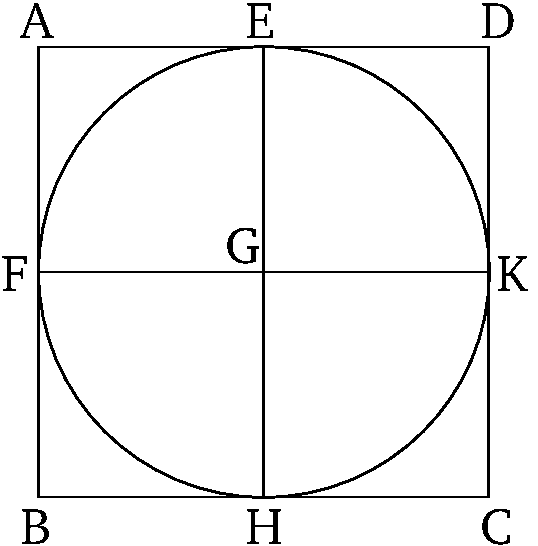
\includegraphics{Book04/fig08e.pdf}}

Let  $AD$ and $AB$ each be cut in half at points $E$ and $F$ (respectively)
[Prop.~1.10]. And let $EH$ be drawn through $E$, parallel
to either of $AB$ or $CD$, and let $FK$ be drawn through $F$, parallel to either of $AD$ or $BC$ [Prop.~1.31].
Thus, $AK$, $KB$, $AH$, $HD$, $AG$, $GC$, $BG$, and $GD$ are each parallelograms,
and their opposite sides [are] manifestly equal [Prop.~1.34].
And since $AD$ is equal to $AB$, and $AE$ is half of $AD$, and $AF$ half of
$AB$, $AE$ (is) thus also equal to $AF$. So that the opposite (sides are) also (equal).
Thus, $FG$ (is) also equal to $GE$. So, similarly, we can also show that each of
$GH$ and $GK$ is equal to each of $FG$ and $GE$. Thus, the four (straight-lines)
$GE$, $GF$, $GH$, and $GK$ [are] equal to one another. Thus, the circle drawn
with center $G$, and radius one of $E$, $F$, $H$, or $K$, will also go through the remaining points. And it will touch the straight-lines $AB$, $BC$, $CD$, and $DA$,
on account of the angles at $E$, $F$, $H$, and $K$ being right-angles. For if the
circle cuts $AB$, $BC$, $CD$, or $DA$, (then) a (straight-line) drawn at right-angles to a diameter of the circle, from its extremity, will fall inside the circle. 
The very thing was shown (to be) absurd [Prop.~3.16].  Thus, the
circle drawn with center $G$, and radius one of $E$, $F$, $H$, or $K$, does not
cut the straight-lines $AB$, $BC$, $CD$, or $DA$. Thus, it will touch them, and will
be inscribed in the square $ABCD$.

Thus, a circle has been inscribed in the given square. (Which is) the very thing it was required to do.}
\end{Parallel}

%%%%%%
% Prop 4.9
%%%%%%
\pdfbookmark[1]{Proposition 4.9}{pdf4.9}
\begin{Parallel}{}{} 
\ParallelLText{
\begin{center}
{\large \ggn{9}.}
\end{center}\vspace*{-7pt}

\gr{Περὶ τὸ δοθὲν τετράγωνον κύκλον περιγράψαι.}

\gr{>'Εστω τὸ δοθὲν τετράγωνον τὸ ΑΒΓΔ; δεῖ δὴ περὶ τὸ ΑΒΓΔ τετράγωνον κύκλον περιγράψαι.}

\gr{Ἐπιζευθθεῖσαι γὰρ αἱ ΑΓ, ΒΔ τεμνέτωσαν ἀλλήλαξ κατὰ τὸ Ε.}

% Removed epsf size command
\centerline{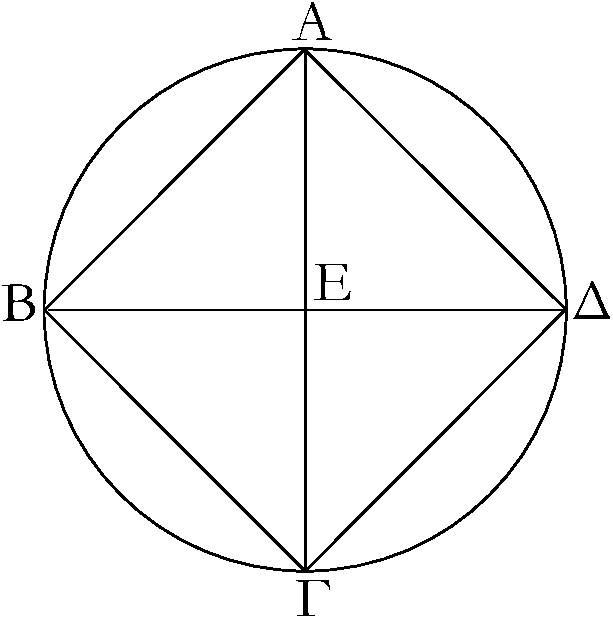
\includegraphics{Book04/fig06g.pdf}}

\gr{Καὶ ἐπεὶ >ίση ἐστὶν ἡ ΔΑ τῆ| ΑΒ, κοινὴ δὲ ἡ ΑΓ, δύο
δὴ αἱ ΔΑ, ΑΓ δυσὶ ταῖξ ΒΑ, ΑΓ >ίσαι εἰσίν; καὶ βάσιξ ἡ ΔΓ βάσει
τῆ| ΒΓ >ίση; γωνία >άρα ἡ ὑπὸ ΔΑΓ γωνίᾳ τῆ| ὑπὸ ΒΑΓ >ίση
ἐστίν; ἡ >άρα ὑπὸ ΔΑΒ γωνία δίθα τέτμ\kern -.7pt  ηται ὑπὸ τῆξ ΑΓ. ὁμοίωξ
δὴ δείχομεν, <ότι καὶ ἑκάστη τῶν ὑπὸ ΑΒΓ, ΒΓΔ, ΓΔΑ δίθα
τέτμ\kern -.7pt  ηται ὑπὸ τῶν ΑΓ, ΔΒ εὐθειῶν. καὶ ἐπεὶ >ίση
ἐστὶν ἡ ὑπὸ ΔΑΒ γωνία τῆ| ὑπὸ ΑΒΓ, καί ἐστι τῆξ μὲν ὑπὸ
ΔΑΒ ἡμίσεια ἡ ὑπὸ ΕΑΒ, τῆξ  δὲ ὑπὸ ΑΒΓ ἡμίσεια ἡ ὑπὸ
ΕΒΑ, καὶ ἡ ὑπὸ ΕΑΒ >άρα τῆ| ὑπὸ ΕΒΑ ἐστιν >ίση; <ώστε
καὶ πλευρὰ ἡ ΕΑ τῆ| ΕΒ ἐστιν >ίση. ὁμοίωξ δὴ δείχομεν,
<ότι καὶ ἑκατέρα τῶν ΕΑ, ΕΒ [εὐθειῶν] ἑκατέρᾳ τῶν ΕΓ, ΕΔ
>ίση ἐστίν. αἱ τέσσαρεξ >άρα αἱ ΕΑ,  ΕΒ, ΕΓ, ΕΔ >ίσαι ἀλλήλαιξ
εἰσίν. ὁ >άρα κέντρῳ τῶ| Ε καὶ διαστήματι ἑνὶ τῶν Α, Β, Γ, Δ
κύκλοξ γραφόμενοξ <ήχει καὶ διὰ τῶν λοιπῶν σημείων καὶ
>έσται περιγεγραμμένοξ περὶ τὸ ΑΒΓΔ τετράγωνον. περιγεγράφθω
ὡξ ὁ ΑΒΓΔ.}

\gr{Περὶ τὸ δοθὲν >άρα τετράγωνον κύκλοξ περιγέγραπται; <όπερ >έδει ποιῆσαι.}}

\ParallelRText{
\begin{center}
{\large Proposition 9}
\end{center}

To  circumscribe a circle about a given square.

Let $ABCD$ be the given square. So it is required to circumscribe a circle about
square $ABCD$.

$AC$ and $BD$ being joined, let them cut one another at $E$.\\

% Removed epsf size command
\centerline{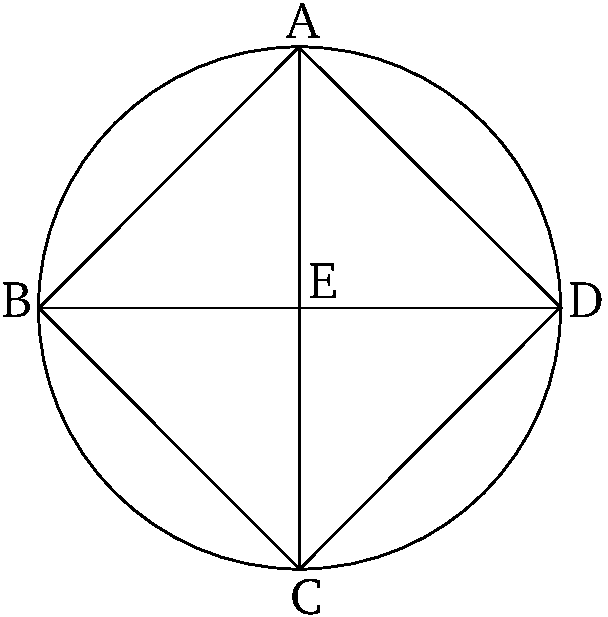
\includegraphics{Book04/fig06e.pdf}}

And since $DA$ is equal to $AB$, and $AC$ (is) common, the two (straight-lines)
$DA$, $AC$ are thus equal to the two (straight-lines) $BA$, $AC$. And the base $DC$
(is) equal to the base $BC$. Thus, angle $DAC$ is equal to angle $BAC$ [Prop.~1.8]. Thus, the angle $DAB$ has been cut in half by $AC$. So, similarly,
we can show that $ABC$, $BCD$, and $CDA$ have each been cut in half
by the straight-lines $AC$ and $DB$. And since angle $DAB$ is equal
 to $ABC$, and $EAB$ is half of $DAB$, and $EBA$ half of $ABC$, $EAB$ is thus
 also equal to $EBA$. So that side $EA$ is also equal to  $EB$ [Prop.~1.6]. So, similarly, we can show that each of the [straight-lines] $EA$ and $EB$ are also equal to each of $EC$ and $ED$. Thus, the four (straight-lines)
 $EA$, $EB$, $EC$, and $ED$ are equal to one another. Thus, the circle drawn with
 center $E$, and radius one of $A$, $B$, $C$, or $D$, will also go through the remaining points, and will be circumscribed about the square $ABCD$. Let
 it be (so) circumscribed, like $ABCD$ (in the figure).
 
 Thus, a circle has been circumscribed about the given square.
 (Which is) the very thing it was required to do.}
\end{Parallel}

%%%%%%
% Prop 4.10
%%%%%%
\pdfbookmark[1]{Proposition 4.10}{pdf4.10}
\begin{Parallel}{}{} 
\ParallelLText{
\begin{center}
{\large \ggn{10}.}
\end{center}\vspace*{-7pt}

\gr{Ἰσοσκελὲξ τρίγωνον συστήσασθαι >έθον ἑκατέραν τῶν πρὸξ τῆ|
βάσει γωνιῶν διπλασίονα τῆξ λοιπῆξ.}

% Removed epsf size command
\centerline{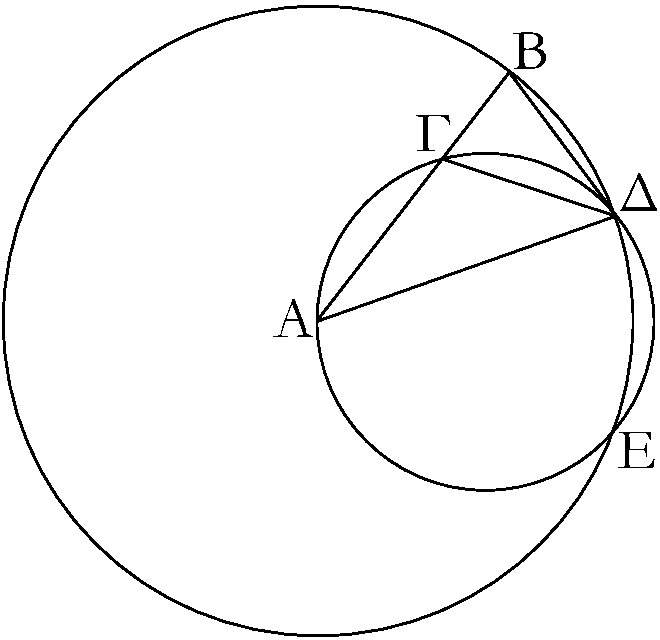
\includegraphics{Book04/fig10g.pdf}}

\gr{Ἐκκείσθω τιξ εὐθεῖα ἡ ΑΒ, καὶ τετμ\kern -.7pt  ήσθω κατὰ τὸ Γ σημεῖον,
<ώστε τὸ ὑπὸ τῶν ΑΒ, ΒΓ περιεχόμενον ὀρθογώνιον >ίσον
ε>ῖναι τῶ| ἀπὸ τῆξ ΓΑ τετραγώνῳ; καὶ κέντρῳ τῶ| Α καὶ
διαστήματι τῶ| ΑΒ κύκλοξ γεγράφθω ὁ ΒΔΕ, καὶ ἐνηρμόσθω
εἰξ τὸν ΒΔΕ κύκλον τῆ| ΑΓ εὐθείᾳ μ\kern -.7pt  ὴ μείζονι ο>ύσῃ τῆξ
τοῦ ΒΔΕ κύκλου διαμέτρου >ίση εὐθεῖα ἡ ΒΔ; καὶ ἐπεζεύθθωσαν
αἱ ΑΔ, ΔΓ, καὶ περιγεγράφθω περὶ τὸ ΑΓΔ τρίγωνον κύκλοξ ὁ
ΑΓΔ.}

\gr{Καὶ ἐπεὶ τὸ ὑπὸ τῶν ΑΒ, ΒΓ >ίσον ἐστὶ τῶ| ἀπὸ
τῆξ ΑΓ, >ίση δὲ ἡ ΑΓ τῆ| ΒΔ, τὸ >άρα ὑπὸ τῶν ΑΒ, ΒΓ >ίσον
ἐστὶ τῶ| ἀπὸ τῆξ ΒΔ. καὶ ἐπεὶ κύκλου τοῦ ΑΓΔ ε>ίληπταί
τι σημεῖον ἐκτὸξ τὸ Β, καὶ ἀπὸ τοῦ Β πρὸξ τὸν ΑΓΔ κύκλον
προσπεπτώκασι δύο εὐθεῖαι αἱ ΒΑ, ΒΔ, καὶ ἡ μὲν α\kern -.7pt  ὐτῶν
τέμνει, ἡ δὲ προσπίπτει, καί ἐστι τὸ ὑπὸ τῶν ΑΒ, ΒΓ >ίσον τῶ| ἀπὸ τῆξ ΒΔ, ἡ ΒΔ >άρα ἐφάπτεται τοῦ ΑΓΔ κύκλου.
ἐπεὶ ο>ῦν ἐφάπτεται μὲν ἡ ΒΔ, ἀπὸ δὲ τῆξ κατὰ τὸ Δ
ἐπαφῆξ διῆκται ἡ ΔΓ, ἡ >άρα ὑπὸ ΒΔΓ γωνιά >ίση ἐστὶ
τῆ| ἐν τῶ| ἐναλλὰχ τοῦ κύκλου τμ\kern -.7pt  ήματι γωνίᾳ
τῆ| ὑπὸ ΔΑΓ. ἐπεὶ ο>ῦν >ίση ἐστὶν ἡ ὑπὸ ΒΔΓ τῆ|
ὑπὸ ΔΑΓ, κοινὴ προσκείσθω ἡ ὑπὸ ΓΔΑ; <όλη >άρα ἡ
ὑπὸ ΒΔΑ >ίση ἐστὶ δυσὶ ταῖξ ὑπὸ ΓΔΑ, ΔΑΓ. ἀλλὰ ταῖξ
ὑπὸ ΓΔΑ, ΔΑΓ >ίση ἐστὶν ἡ ἐκτὸξ ἡ ὑπὸ ΒΓΔ;
καὶ ἡ ὑπὸ ΒΔΑ >άρα >ίση ἐστὶ τῆ| ὑπὸ ΒΓΔ. ἀλλὰ
ἡ ὑπὸ ΒΔΑ τῆ| ὑπὸ ΓΒΔ ἐστιν >ίση, ἐπεὶ καὶ πλευρὰ
ἡ ΑΔ τῆ| ΑΒ ἐστιν >ίση; <ώστε καὶ ἡ ὑπὸ ΔΒΑ τῆ|
ὑπὸ ΒΓΔ ἐστιν >ίση.
αἱ τρεῖξ >άρα αἱ ὑπὸ ΒΔΑ,
ΔΒΑ, ΒΓΑ >ίσαι ἀλλήλαιξ εἰσίν. καὶ ἐπεὶ >ίση ἐστὶν
ἡ ὑπὸ ΔΒΓ γωνία τῆ| ὑπὸ ΒΓΔ, >ίση ἐστὶ καὶ πλευρὰ
ἡ ΒΔ πλευρᾶ| τῆ| ΔΓ. ἀλλὰ ἡ ΒΔ τῆ| ΓΑ ὑπόκειται >ίση;
καὶ ἡ ΓΑ >άρα τῆ| ΓΔ ἐστιν >ίση; <ώστε καὶ
γωνία ἡ ὑπὸ ΓΔΑ γωνίᾳ τῆ| ὑπὸ ΔΑΓ ἐστιν >ίση; αἱ
>άρα ὑπὸ ΓΔΑ, ΔΑΓ τῆξ ὑπὸ ΔΑΓ εἰσι διπλασίουξ.
>ίση δὲ ἡ ὑπὸ ΒΓΔ ταῖξ ὑπὸ ΓΔΑ, ΔΑΓ; καὶ
ἡ ὑπὸ ΒΓΔ >άρα τῆξ ὑπὸ ΓΑΔ ἐστι διπλῆ. >ίση
δὲ ἡ ὑπὸ ΒΓΔ ἑκατέρᾳ τῶν ὑπὸ ΒΔΑ, ΔΒΑ; καὶ
ἑκατέρα >άρα τῶν ὑπὸ ΒΔΑ, ΔΒΑ τῆξ ὑπὸ ΔΑΒ
ἐστι διπλῆ.}

\gr{Ἰσοσκελὲξ >άρα τρίγωνον συνέσταται τὸ ΑΒΔ >έθον
ἑκατέραν τῶν πρὸξ τῆ| ΔΒ βάσει γωνιῶν διπλασίονα τῆξ
λοιπῆξ; <όπερ >έδει ποιῆσαι.}}

\ParallelRText{
\begin{center}
{\large Proposition 10}
\end{center}

To construct an isosceles triangle having each of the angles at the base
double the remaining (angle).

% Removed epsf size command
\centerline{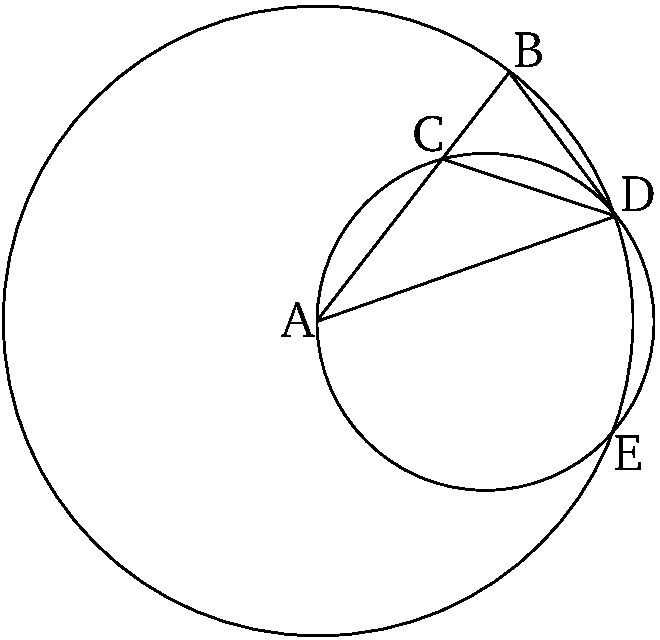
\includegraphics{Book04/fig10e.pdf}}

Let some straight-line $AB$ be taken, and let it be cut at point $C$
so that the rectangle contained by $AB$ and $BC$ is equal to the square
on $CA$ [Prop.~2.11]. And let the circle $BDE$ be drawn with
center $A$, and radius $AB$. And let the straight-line $BD$, equal to the straight-line $AC$, being not greater than the diameter of circle $BDE$, be inserted into circle $BDE$ [Prop.~4.1]. And let $AD$ and $DC$ be joined. 
And let the circle $ACD$ be circumscribed about triangle $ACD$ [Prop.~4.5].

And since the (rectangle contained) by $AB$ and $BC$ is equal to the
(square) on $AC$, and $AC$ (is) equal to $BD$, the (rectangle contained) by
$AB$ and $BC$ is thus equal to the (square) on $BD$. And since some point
$B$ has been taken outside of circle $ACD$, and two straight-lines $BA$ and
$BD$ have radiated from $B$ towards the circle $ACD$, and (one) of them
cuts (the circle), and (the other) meets (the circle), and the (rectangle contained)
by $AB$ and $BC$ is equal to the (square) on  $BD$,   $BD$ thus touches
circle $ACD$ [Prop.~3.37]. Therefore, since $BD$ touches (the circle),
and $DC$ has been drawn across (the circle) from the point of contact $D$,
the angle $BDC$ is thus equal to the angle $DAC$ in the alternate segment
of the circle [Prop.~3.32]. Therefore, since $BDC$ is equal to
$DAC$, let $CDA$ be added to both. Thus, the whole of $BDA$ is equal
to the two (angles) $CDA$ and $DAC$. But, the
external (angle)  $BCD$  is equal to $CDA$ and $DAC$  [Prop.~1.32]. Thus, $BDA$ is also equal to
$BCD$. But, $BDA$ is equal to $CBD$, since the side $AD$ is also equal to
$AB$ [Prop.~1.5]. So that $DBA$ is also equal to $BCD$. Thus, the three
(angles) $BDA$, $DBA$, and $BCD$ are equal to one another. And since angle
$DBC$ is equal to $BCD$, side $BD$ is also equal to side $DC$ [Prop.~1.6].
But, $BD$ was assumed (to be) equal to $CA$. Thus, $CA$ is also equal to $CD$.
So that angle $CDA$ is also equal to angle $DAC$ [Prop.~1.5]. 
Thus, $CDA$ and $DAC$ is double $DAC$. But $BCD$ (is) equal to $CDA$ and
$DAC$. Thus, $BCD$ is also double $CAD$. And $BCD$ (is) equal to to each of
$BDA$ and $DBA$. Thus, $BDA$ and $DBA$ are each double $DAB$.

Thus, the isosceles triangle $ABD$ has been constructed having each of the
angles at the base $BD$ double the remaining (angle). (Which is) the
very thing it was required to do.}
\end{Parallel}

%%%%%%
% Prop 4.11
%%%%%%
\pdfbookmark[1]{Proposition 4.11}{pdf4.11}
\begin{Parallel}{}{} 
\ParallelLText{
\begin{center}
{\large \ggn{11}.}
\end{center}\vspace*{-7pt}

\gr{Εἰξ τὸν δοθέντα κύκλον πεντάγωνον ἰσόπλευρόν τε καὶ ἰσογώνιον
ἐγγράψαι.}

% Removed epsf size command
\centerline{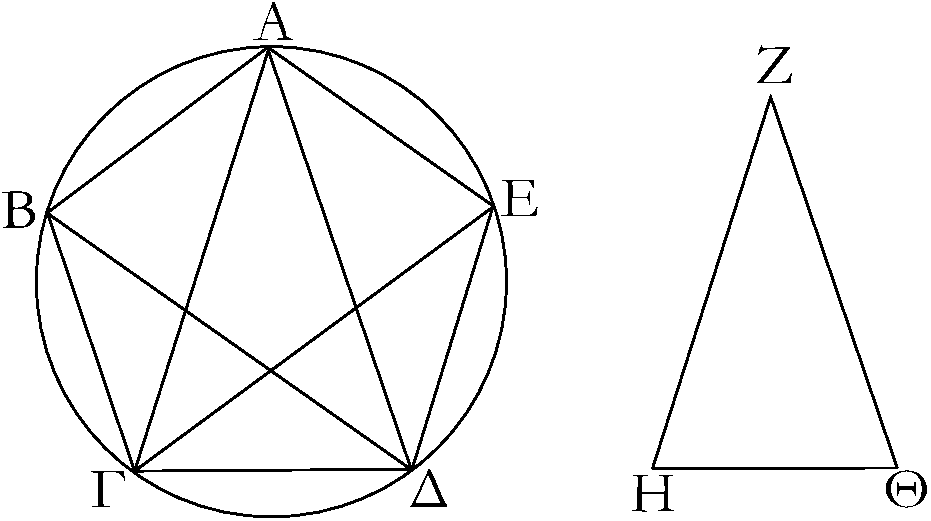
\includegraphics{Book04/fig11g.pdf}}

\gr{>'Εστω ὁ δοθεὶξ κύκλοξ ὁ ΑΒΓΔΕ; δεῖ δὴ εἰξ τὸν ΑΒΓΔΕ κύκλον πεντάγωνον ἰσόπλευρόν τε καὶ ἰσογώνιον ἐγγράψαι.}

\gr{Ἐκκείσθω τρίγωνον ἰσοσκελὲξ τὸ ΖΗΘ διπλασίονα >έθον ἑκατέραν
τῶν πρὸξ τοῖξ Η, Θ γωνιῶν τῆξ πρὸξ τῶ| Ζ, καὶ ἐγγεγράφθω
εἰξ τὸν ΑΒΓΔΕ κύκλον τῶ| ΖΗΘ τριγώνῳ ἰσογώνιον τρίγωνον
τὸ ΑΓΔ, <ώστε τῆ| μὲν πρὸξ τῶ| Ζ γωνίᾳ >ίσην ε>ῖναι
τὴν ὑπὸ ΓΑΔ, ἑκατέραν δὲ τῶν πρὸξ τοῖξ Η, Θ >ίσην ἑκατέρᾳ
τῶν ὑπὸ ΑΓΔ, ΓΔΑ; καὶ ἑκατέρα >άρα τῶν ὑπὸ ΑΓΔ, ΓΔΑ
τῆξ ὑπὸ ΓΑΔ ἐστι διπλῆ. τετμ\kern -.7pt  ήσθω δὴ ἑκατέρα τῶν ὑπὸ
ΑΓΔ, ΓΔΑ δίθα ὑπὸ ἑκατέραξ τῶν ΓΕ, ΔΒ εὐθειῶν, καὶ
ἐπεζεύθθωσαν αἱ ΑΒ, ΒΓ,  ΔΕ, ΕΑ.}

\gr{Ἐπεὶ ο>ῦν ἑκατέρα τῶν ὑπὸ ΑΓΔ, ΓΔΑ γωνιῶν διπλασίων
ἐστὶ τῆξ ὑπὸ ΓΑΔ, καὶ τετμ\kern -.7pt  ημέναι εἰσὶ δίθα ὑπὸ τῶν ΓΕ,
ΔΒ εὐθειῶν, αἱ πέντε >άρα γωνίαι αἱ ὑπὸ ΔΑΓ, ΑΓΕ, ΕΓΔ, ΓΔΒ,
ΒΔΑ >ίσαι ἀλλήλαιξ εἰσίν. αἱ δὲ >ίσαι γωνίαι ἐπὶ >ίσων
περιφερειῶν βεβήκασιν; αἱ πέντε  >άρα περιφέρειαι αἱ ΑΒ, ΒΓ, ΓΔ, ΔΕ, ΕΑ >ίσαι ἀλλήλαιξ εἰσίν. ὑπὸ δὲ τὰξ >ίσαξ
περιφερείαξ >ίσαι εὐθεῖαι ὑποτείνουσιν; αἱ πέντε >άρα εὐθεῖαι
αἱ ΑΒ, ΒΓ, ΓΔ, ΔΕ, ΕΑ >ίσαι ἀλλήλαιξ εἰσίν; ἰσόπλευρον >άρα
ἐστὶ τὸ ΑΒΓΔΕ πεντάγωνον. λέγω δή, <ότι καὶ ἰσογώνιον. ἐπεὶ
γὰρ ἡ ΑΒ περιφέρεια τῆ| ΔΕ περιφερείᾳ ἐστὶν >ίση, κοινὴ
προσκείσθω ἡ ΒΓΔ; <όλη >άρα ἡ ΑΒΓΔ περιφέρια  <όλῃ
τῆ| ΕΔΓΒ
περιφερείᾳ ἐστὶν >ίση. καὶ βέβηκεν ἐπὶ μὲν τῆξ ΑΒΓΔ
περιφερείαξ γωνία ἡ ὑπὸ ΑΕΔ, ἐπὶ δὲ τῆξ ΕΔΓΒ περιφερείαξ
γωνία ἡ ὑπὸ ΒΑΕ; καὶ ἡ ὑπὸ ΒΑΕ >άρα γωνία
τῆ| ὑπὸ ΑΕΔ ἐστιν >ίση. διὰ τὰ α\kern -.7pt  ὐτὰ δὴ καὶ ἑκάστη τῶν
ὑπὸ ΑΒΓ, ΒΓΔ, ΓΔΕ γωνιῶν ἑκατέρᾳ τῶν ὑπὸ ΒΑΕ, ΑΕΔ
ἐστιν >ίση; ἰσογώνιον >άρα ἐστὶ τὸ ΑΒΓΔΕ πεντάγωνον.
ἐδείθθη δὲ καὶ ἰσόπλευρον.}

\gr{Εἰξ >άρα τὸν δοθέντα κύκλον πεντάγωνον ἰσόπλευρόν τε καὶ ἰσογώνιον
ἐγγέγραπται; <όπερ >έδει ποιῆσαι.}}

\ParallelRText{
\begin{center}
{\large Proposition 11}
\end{center}

To inscribe an equilateral and equiangular pentagon in a given circle.

% Removed epsf size command
\centerline{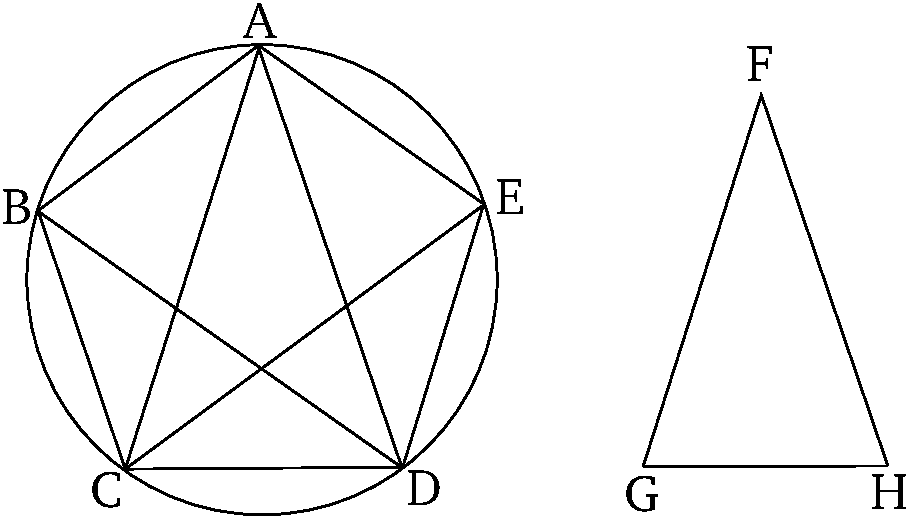
\includegraphics{Book04/fig11e.pdf}}

Let $ABCDE$ be the given circle. So it is required to inscribed an equilateral
and equiangular pentagon in circle $ABCDE$.

Let the the isosceles triangle $FGH$ be set up having each of the angles
at $G$ and $H$ double the (angle) at $F$ [Prop.~4.10]. And let triangle $ACD$, equiangular
to $FGH$, be inscribed in circle $ABCDE$, such that $CAD$ is equal 
to the angle at $F$, and  the (angles) at $G$ and $H$ (are) equal to $ACD$ and $CDA$, respectively [Prop.~4.2]. Thus,
$ACD$ and $CDA$ are each double $CAD$. So let $ACD$ and $CDA$ 
be cut in half by the straight-lines $CE$ and $DB$, respectively
[Prop.~1.9]. And let $AB$, $BC$, $DE$ and
$EA$ be joined.

Therefore, since angles $ACD$ and $CDA$ are each double $CAD$, and are cut
in half by the straight-lines $CE$ and $DB$, the five angles
$DAC$, $ACE$, $ECD$, $CDB$, and $BDA$ are thus equal to one another.
And equal angles stand upon equal circumferences [Prop.~3.26]. Thus, the five circumferences
$AB$, $BC$, $CD$, $DE$, and $EA$ are equal to one another [Prop.~3.29]. Thus, the pentagon
$ABCDE$ is equilateral. So I say that (it is) also equiangular. For since the
circumference $AB$ is equal to the circumference $DE$, let $BCD$ be added to both. Thus, the whole circumference $ABCD$ is equal to the
whole circumference $EDCB$. And the angle $AED$ stands upon circumference
$ABCD$, and angle $BAE$ upon circumference $EDCB$. Thus, angle $BAE$ is
also equal to $AED$ [Prop.~3.27]. 
So, for the same (reasons), each of the angles $ABC$, $BCD$,  and $CDE$ is also equal
to each of $BAE$ and $AED$. Thus, pentagon $ABCDE$ is equiangular.
And it was also shown (to be) equilateral.

Thus, an equilateral and equiangular pentagon has been inscribed in the
given circle. (Which is) the very thing it was required to do.}
\end{Parallel}

%%%%%%
% Prop 4.12
%%%%%%
\pdfbookmark[1]{Proposition 4.12}{pdf4.12}
\begin{Parallel}{}{} 
\ParallelLText{
\begin{center}
{\large \ggn{12}.}
\end{center}\vspace*{-7pt}

\gr{Περὶ τὸν δοθέντα κύκλον πεντάγωνον ἰσόπλευρόν τε καὶ ἰσογώνιον
περιγράψαι.}

% Removed epsf size command
\centerline{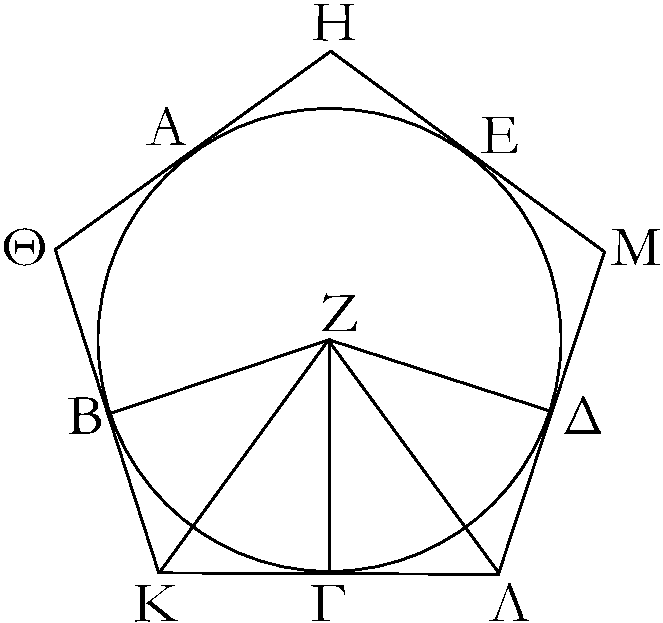
\includegraphics{Book04/fig12g.pdf}}

\gr{>'Εστω ὁ δοθεὶξ κύκλοξ ὁ ΑΒΓΔΕ; δεῖ δὲ περὶ τὸν ΑΒΓΔΕ κύκλον
πεντάγωνον ἰσόπλευρόν τε καὶ ἰσογώνιον περιγράψαι.}

\gr{Νενοήσθω τοῦ ἐγγεγραμμένου πενταγώνου τῶν γωνιῶν σημεῖα
τὰ Α, Β, Γ, Δ, Ε, <ώστε >ίσαξ ε>ῖναι τὰξ ΑΒ, ΒΓ, ΓΔ, ΔΕ, ΕΑ
περιφερείαξ; καὶ διὰ τῶν Α, Β, Γ, Δ, Ε >ήθθωσαν τοῦ κύκλου
ἐφαπτόμεναι αἱ ΗΘ, ΘΚ, ΚΛ, ΛΜ, μ\kern -.7pt  η, καὶ εἰλήφθω τοῦ ΑΒΓΔΕ
κύκλου κέντρον τὸ Ζ, καὶ ἐπεζεύθθωσαν αἱ ΖΒ, ΖΚ, ΖΓ, ΖΛ, ΖΔ.}

\gr{Καὶ ἐπεὶ ἡ μὲν ΚΛ εὐθεῖα ἐφάπτεται τοῦ ΑΒΓΔΕ κατὰ τὸ
Γ, ἀπὸ δὲ τοῦ Ζ κέντρου ἐπὶ τὴν κατὰ τὸ Γ ἐπαφὴν ἐπέζευκται
ἡ ΖΓ, ἡ ΖΓ >άρα κάθετόξ ἐστιν ἐπὶ τὴν ΚΛ; ὀρθὴ >άρα ἐστὶν
ἑκατέρα τῶν πρὸξ τῶ| Γ γωνιῶν. διὰ τὰ α\kern -.7pt  ὐτὰ δὴ καὶ αἱ 
πρὸξ τοῖξ Β, Δ σημείοιξ γωνίαι  ὀρθαί εἰσιν. καὶ ἐπεὶ ὀρθή 
ἐστιν ἡ ὑπὸ ΖΓΚ γωνία, τὸ >άρα ἀπὸ τῆξ ΖΚ >ίσον 
ἐστὶ τοῖξ ἀπὸ τῶν ΖΓ, ΓΚ. διὰ τὰ α\kern -.7pt  ὐτὰ δὴ καὶ τοῖξ 
ἀπὸ τῶν ΖΒ, ΒΚ >ίσον ἐστὶ τὸ ἀπὸ τῆξ ΖΚ; <ώστε τὰ ἀπὸ
τῶν ΖΓ, ΓΚ τοῖξ ἀπὸ τῶν ΖΒ, ΒΚ ἐστιν >ίσα, <ῶν τὸ
ἀπὸ τῆξ ΖΓ τῶ| ἀπὸ τῆξ ΖΒ ἐστιν >ίσον; λοιπὸν >άρα
τὸ ἀπὸ τῆξ ΓΚ τῶ| ἀπὸ τῆξ ΒΚ ἐστιν >ίσον. >ίση
>άρα ἡ ΒΚ τῆ| ΓΚ. καὶ ἐπεὶ >ίση ἐστὶν ἡ ΖΒ τῆ| ΖΓ, καὶ κοινὴ 
ἡ ΖΚ, δύο δὴ αἱ ΒΖ, ΖΚ δυσὶ ταῖξ ΓΖ, ΖΚ >ίσαι εἰσίν;
καὶ βάσιξ ἡ ΒΚ βάσει τῆ| ΓΚ [ἐστιν] >ίση; γωνία >άρα ἡ μὲν 
ὑπὸ ΒΖΚ [γωνίᾳ] τῆ| ὑπὸ ΚΖΓ ἐστιν >ίση; ἡ δὲ ὑπὸ ΒΚΖ
τῆ| ὑπὸ ΖΚΓ; διπλῆ >άρα ἡ μὲν ὑπὸ ΒΖΓ τῆξ ὑπὸ ΚΖΓ,
ἡ δὲ ὑπὸ ΒΚΓ τῆξ ὑπὸ ΖΚΓ. διὰ τὰ α\kern -.5pt  ὐτὰ δὴ καὶ ἡ
μὲν ὑπὸ ΓΖΔ τῆξ ὑπὸ ΓΖΛ ἐστι διπλῆ, ἡ δὲ ὑπὸ ΔΛΓ
τῆξ ὑπὸ ΖΛΓ. καὶ ἐπεὶ >ίση ἐστὶν ἡ ΒΓ περιφέρεια τῆ| ΓΔ,
>ίση ἐστὶ καὶ γωνία ἡ ὑπὸ ΒΖΓ τῆ| ὑπὸ ΓΖΔ.
καί ἐστιν ἡ μὲν ὑπὸ ΒΖΓ τῆξ ὑπὸ ΚΖΓ διπλῆ,
ἡ δὲ ὑπὸ ΔΖΓ τῆξ ὑπὸ ΛΖΓ; >ίση >άρα καὶ ἡ ὑπὸ
ΚΖΓ τῆ| ὑπὸ ΛΖΓ; ἐστὶ δὲ καὶ ἡ ὑπὸ ΖΓΚ γωνία
τῆ| ὑπὸ ΖΓΛ >ίση. δύο δὴ τρίγωνά ἐστι τὰ ΖΚΓ,
ΖΛΓ τὰξ  δύο γωνίαξ ταῖξ δυσὶ γωνίαιξ >ίσαξ >έθοντα καὶ
μίαν πλευρὰν μιᾶ| πλευρᾶ| >ίσην κοινὴν α\kern -.3pt  ὐτῶν
τὴν ΖΓ; καὶ τὰξ λοιπὰξ >άρα πλευρὰξ ταῖξ λοιπαῖξ πλευραῖξ >ίσαξ
<έχει καὶ τὴν λοιπὴν γωνίαν τῆ| λοιπῆ| γωνίᾳ; >ίση >άρα ἡ μὲν ΚΓ εὐθεῖα τῆ| ΓΛ, ἡ δὲ ὑπὸ
ΖΚΓ γωνία τῆ| ὑπὸ ΖΛΓ. καὶ ἐπεὶ >ίση ἐστὶν
ἡ ΚΓ τῆ| ΓΛ, διπλῆ >άρα ἡ ΚΛ τῆξ ΚΓ. διὰ τὰ α\kern -.7pt  ὐτα
δὴ δειθθήσεται καὶ ἡ 
ΘΚ τῆξ ΒΚ διπλῆ. καί ἐστιν ἡ ΒΚ τῆ| ΚΓ
>ίση; καὶ ἡ ΘΚ >άρα τῆ| ΚΛ ἐστιν >ίση. ὁμοίωξ δὴ δειθθήσεται
καὶ ἑκάστη τῶν ΘΗ, ΗΜ,
ΜΛ ἑκατέρᾳ τῶν ΘΚ, ΚΛ >ίση; ἰσόπλευρον >άρα ἐστὶ τὸ ΗΘΚΛΜ
πεντάγωνον. λέγω δή, <ότι καὶ ἰσογώνιον. ἐπεὶ γὰρ >ίση
ἐστὶν ἡ ὑπὸ ΖΚΓ γωνία τῆ| ὑπὸ ΖΛΓ, καὶ ἐδείθθη τῆξ
μὲν ὑπὸ ΖΚΓ διπλῆ ἡ ὑπὸ
ΘΚΛ, τῆξ δὲ ὑπὸ ΖΛΓ διπλῆ ἡ ὑπὸ ΚΛΜ, καὶ ἡ ὑπὸ
ΘΚΛ >άρα τῆ| ὑπὸ ΚΛΜ ἐστιν >ίση. ὁμοίωξ δὴ δειθθήσεται καὶ
ἑκάστη τῶν ὑπὸ ΚΘΗ, ΘΗΜ, ΗΜΛ ἑκατέρᾳ τῶν ὑπὸ ΘΚΛ, ΚΛΜ
>ίση; αἱ πέντε >άρα γωνίαι αἱ ὑπὸ ΗΘΚ, ΘΚΛ, ΚΛΜ, Λμ\kern -.7pt  η,
μ\kern -.7pt  ηΘ
>ίσαι ἀλλήλαιξ εἰσίν. ἰσογώνιον >άρα ἐστὶ τὸ ΗΘΚΛΜ
πεντάγωνον. ἐδείθθη δὲ καὶ ἰσόπλευρον, καὶ
περιγέγραπται περὶ τὸν ΑΒΓΔΕ κύκλον.}

\gr{\kern -.7pt {[}Per`i t`on doj'enta >'ara k'uklon pent'agwnon >is'opleur\-'on
te ka`i >isog'wnion perig'egraptai]; <'oper >'edei
poi~hsai.}}

\ParallelRText{
\begin{center}
{\large Proposition 12}
\end{center}

To circumscribe an equilateral and equiangular
pentagon about a given circle.

% Removed epsf size command
\centerline{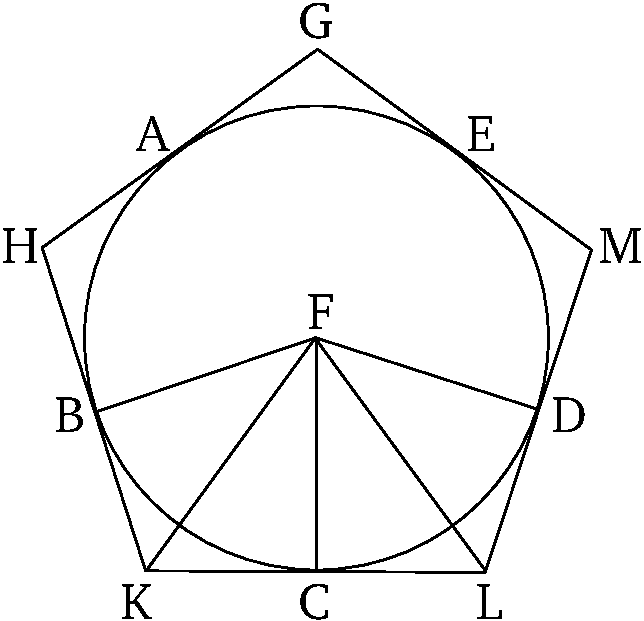
\includegraphics{Book04/fig12e.pdf}}

Let $ABCDE$ be the given circle. So it is required to circumscribe an
equilateral and equiangular pentagon about circle $ABCDE$. 

Let $A$, $B$, $C$, $D$,  and $E$ be conceived as the angular points of a
pentagon having been inscribed (in circle $ABCDE$) [Prop.~3.11], such that the circumferences $AB$, $BC$, $CD$, $DE$, and
$EA$ are equal. And let $GH$, $HK$, $KL$, $LM$, and $MG$  be drawn through
(points) $A$, $B$, $C$, $D$, and $E$ (respectively), touching the circle.$^\dag$ And let the center $F$
of the circle $ABCDE$ be found [Prop.~3.1].
And let $FB$, $FK$, $FC$, $FL$, and $FD$ be joined.

And since the straight-line $KL$ touches (circle) $ABCDE$ at $C$, and $FC$ has been
joined from the center $F$ to the point of contact $C$, $FC$ is thus perpendicular 
to $KL$ [Prop.~3.18]. Thus, each of the angles
at $C$ is a right-angle. So, for the same (reasons), the angles at $B$ and $D$
are also right-angles. And since angle $FCK$ is a right-angle, the (square)
on $FK$ is thus equal to the (sum of the squares) on $FC$ and $CK$ [Prop.~1.47]. So, for the same (reasons), 
the (square) on $FK$ is also equal to the (sum of the squares) on $FB$ and $BK$.
So that the (sum of the squares) on $FC$ and $CK$ is equal to the (sum of the squares) on $FB$ and $BK$, of which the (square) on $FC$ is equal to the
(square) on $FB$. Thus, the remaining (square) on $CK$ is equal to
the remaining (square) on $BK$. Thus, $BK$ (is) equal to $CK$. And since
$FB$ is equal to $FC$, and $FK$ (is) common, the two (straight-lines)
$BF$, $FK$ are equal to the two (straight-lines) $CF$, $FK$. And the base $BK$
[is] equal to the base $CK$. Thus, angle $BFK$ is equal to [angle] $KFC$ 
[Prop.~1.8]. And $BKF$ (is equal) to $FKC$ [Prop.~1.8].
Thus, $BFC$ (is) double $KFC$,
and $BKC$ (is double) $FKC$. So, for the same (reasons), $CFD$ is also double
$CFL$, and $DLC$ (is also double) $FLC$. And since circumference $BC$
is equal  to $CD$, angle $BFC$ is also  equal  to $CFD$ [Prop.~3.27]. And $BFC$ is double $KFC$,
and $DFC$ (is double) $LFC$.  Thus, $KFC$ is also equal to $LFC$. 
And
angle $FCK$ is also equal to $FCL$. So, $FKC$ and $FLC$ are two triangles
having two angles equal to two angles, and one side equal to one side,
(namely) their common (side) $FC$. Thus, they will also have the
remaining sides equal to the (corresponding) remaining sides, and
the remaining angle to the remaining angle [Prop.~1.26]. Thus, the straight-line $KC$
(is) equal to $CL$, and the angle $FKC$ to $FLC$. And since $KC$ is
equal to $CL$, $KL$ (is) thus double $KC$. So, for the
same (reasons), it can be shown that $HK$ (is) also double $BK$. And
$BK$ is equal to $KC$. Thus, $HK$ is also equal to $KL$. So, similarly,  each of $HG$, $GM$, and $ML$ can also be shown (to be) equal to each of
$HK$ and $KL$. Thus, pentagon $GHKLM$ is equilateral. So I say that
(it is) also equiangular. For since angle $FKC$ is equal to $FLC$, 
and $HKL$ was shown (to be) double $FKC$, and $KLM$ double 
$FLC$, $HKL$ is thus also equal to $KLM$. So, similarly, each of $KHG$, $HGM$, and $GML$ can also be shown (to be) equal to each of
$HKL$ and $KLM$. Thus, the five angles $GHK$, $HKL$, $KLM$, $LMG$, and
$MGH$ are equal to one another. Thus, the pentagon $GHKLM$ is
equiangular. And it was also shown (to be) equilateral, and has been circumscribed 
about circle $ABCDE$.

\mbox{[}Thus, an equilateral and equiangular pentagon has been circumscribed
about the given circle]. (Which is) the very thing it was required to do. }
\end{Parallel}
{\footnotesize \noindent$^\dag$ See the footnote to Prop.~3.34.} 

%%%%%%
% Prop 4.13
%%%%%%
\pdfbookmark[1]{Proposition 4.13}{pdf4.13}
\begin{Parallel}{}{} 
\ParallelLText{
\begin{center}
{\large \ggn{13}.}
\end{center}\vspace*{-7pt}

\gr{Εἰξ τὸ δοθὲν πεντάγωνον, <ό ἐστιν ἰσόπλευρόν τε καὶ ἰσογώνιον, κύκλον ἐγγράψαι.}

\gr{>'Εστω τὸ δοθὲν πεντάγωνον ἰσόπλευρόν τε καὶ ἰσογώνι\-ον
τὸ ΑΒΓΔΕ; δεῖ δὴ εἰξ τὸ ΑΒΓΔΕ πεντάγωνον κύκλον ἐγγράψαι.}

\gr{Τετμ\kern -.7pt  ήσθω γὰρ ἑκατέρα τῶν ὑπὸ ΒΓΔ, ΓΔΕ γωνιῶν δίθα ὑπὸ
ἑκατέραξ τῶν ΓΖ, ΔΖ εὐθειῶν; καὶ ἀπὸ τοῦ Ζ σημείου, καθ> <ὸ
συμβάλλουσιν ἀλλήλαιξ αἱ ΓΖ, ΔΖ εὐθεῖαι, ἐπεζεύθθωσαν αἱ ΖΒ,
ΖΑ, ΖΕ εὐθεῖαι. καὶ ἐπεὶ >ίση ἐστὶν ἡ ΒΓ τῆ| ΓΔ, κοινὴ
δὲ ἡ ΓΖ, δύο δὴ αἱ ΒΓ, ΓΖ δυσὶ ταῖξ ΔΓ, ΓΖ >ίσαι
εἰσίν; καὶ γωνία ἡ ὑπὸ ΒΓΖ γωνίᾳ τῆ| ὑπὸ ΔΓΖ [ἐστιν]
>ίση; βάσιξ >άρα ἡ ΒΖ βάσει τῆ| ΔΖ ἐστιν >ίση, 
καὶ τὸ ΒΓΖ τρίγωνον τῶ| ΔΓΖ τριγώνῳ ἐστιν >ίσον,
καὶ αἱ λοιπαὶ
γωνίαι ταῖξ λοιπαῖξ γωνίαιξ >ίσαι >έσονται, ὑφ> <ὰξ αἱ
>ίσαι πλευραὶ ὑποτείνουσιν; >ίση >άρα ἡ ὑπὸ ΓΒΖ γωνία 
τῆ|  ὑπὸ ΓΔΖ. καὶ ἐπεὶ διπλῆ ἐστιν ἡ ὑπὸ ΓΔΕ τῆξ 
ὑπὸ ΓΔΖ, >ίση δὲ ἡ μὲν ὑπὸ ΓΔΕ τῆ| ὑπὸ ΑΒΓ, ἡ δὲ 
ὑπὸ ΓΔΖ τῆ| ὑπὸ ΓΒΖ, καὶ ἡ ὑπὸ ΓΒΑ >άρα τῆξ ὑπὸ
ΓΒΖ ἐστι διπλῆ; >ίση >άρα ἡ ὑπὸ ΑΒΖ γωνία τῆ| ὑπὸ
ΖΒΓ; ἡ >άρα ὑπὸ ΑΒΓ γωνία δίθα τέτμ\kern -.7pt  ηται ὑπὸ τῆξ
ΒΖ εὐθείαξ. ὁμοίωξ δὴ δειθθήσεται, <ότι καὶ ἑκατέρα τῶν
ὑπὸ ΒΑΕ, ΑΕΔ δίθα τέτμ\kern -.5pt  ηται ὑπὸ ἑκατέραξ τῶν ΖΑ, ΖΕ
εὐθειῶν. >ήθθωσαν δὴ ἀπὸ τοῦ Ζ σημείου ἐπὶ τὰξ ΑΒ, ΒΓ,
ΓΔ, ΔΕ, ΕΑ εὐθείαξ κάθετοι αἱ ΖΗ, ΖΘ, ΖΚ, ΖΛ, ΖΜ. καὶ ἐπεὶ
>ίση ἐστὶν ἡ ὑπὸ ΘΓΖ γωνία τῆ| ὑπὸ ΚΓΖ, ἐστὶ δὲ 
καὶ ὀρθὴ ἡ ὑπὸ ΖΘΓ
[ὀρθῆ|] τῆ| ὑπὸ ΖΚΓ >ίση,
δύο δὴ τρίγωνά ἐστι τὰ ΖΘΓ, ΖΚΓ τὰξ δύο γωνίαξ δυσὶ γωνίαιξ >ίσαξ
>έθοντα καὶ μίαν πλευρὰν μιᾶ| πλευρᾶ| >ίσην κοινὴν α\kern -.3pt  ὐτῶν 
τὴν ΖΓ ὑποτείνουσαν ὑπὸ μίαν τῶν >ίσων γωνιῶν; καὶ
τὰξ λοιπὰξ >άρα πλευρὰξ ταῖξ λοιπαῖξ πλευραῖξ >ίσαξ <έχει;
>ίση >άρα ἡ ΖΘ κάθετοξ τὴ| ΖΚ καθέτῳ. ὁμοίωξ
δὴ δειθθήσεται, <ότι καὶ ἑκάστη τῶν ΖΛ, ΖΜ, ΖΗ
ἑκατέρᾳ τῶν ΖΘ, ΖΚ >ίση ἐστίν; αἱ πέντε >άρα εὐθεῖαι αἱ
ΖΗ, ΖΘ, ΖΚ, ΖΛ, ΖΜ  >ίσαι ἀλλήλαιξ εἰσίν. ὁ >άρα
κέντρῳ τῶ| Ζ διαστήματι δὲ ἑνὶ τῶν Η, Θ, Κ, Λ, Μ
κύκλοξ γραφόμενοξ <ήχει καὶ διὰ τῶν λοιπῶν σημείων
καὶ ἐφάψεται τῶν 
ΑΒ, ΒΓ, ΓΔ, ΔΕ, ΕΑ εὐθειῶν διὰ τὸ ὀρθὰξ ε>ῖναι
τὰξ πρὸξ τοῖξ Η, Θ, Κ, Λ, Μ σημείοιξ γωνίαξ. εἰ γὰρ οὐκ
ἐφάψεται α\kern -.7pt  ὐτῶν, ἀλλὰ τεμεῖ α\kern -.7pt  ὐτάξ, συμβήσεται τὴν τῆ|
διαμέτρῳ τοῦ κύκλου πρὸξ ὀρθὰξ ἀπ> >άκραξ ἀγομένην
ἐντὸξ πίπτειν τοῦ κύκλου; <όπερ >άτοπον ἐδείθθη.
οὐκ >άρα ὁ κέντρῳ τῶ| Ζ διαστήματι δὲ ἑνὶ τῶν
Η, Θ, Κ, Λ, Μ σημείων γραφόμενοξ κύκλοξ τεμεῖ τὰξ ΑΒ, ΒΓ, ΓΔ, ΔΕ,
ΕΑ εὐθείαξ;  ἐφάψεται >άρα α\kern -.7pt  ὐτῶν. γεγράφθω ὡξ ὁ ΗΘΚΛΜ.}\\~\\~\\

% Removed epsf size command
\centerline{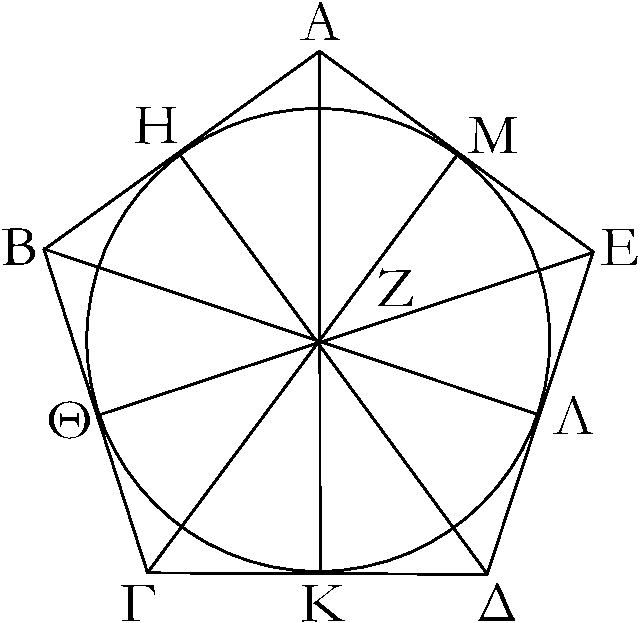
\includegraphics{Book04/fig13g.pdf}}

\gr{Εἰξ >άρα τὸ δοθὲν πεντάγωνον, <ό ἐστιν ἰσόπλευρόν
τε καὶ ἰσογώνιον, κύκλοξ ἐγγέγραπται; <όπερ >έδει ποιῆσαι.}}

\ParallelRText{
\begin{center}
{\large Proposition 13}
\end{center}

To inscribe a circle in a given
pentagon, which is equilateral and equiangular.

Let $ABCDE$ be the given equilateral and equiangular pentagon. So
it is required to inscribe a circle in pentagon $ABCDE$.

For let angles $BCD$ and $CDE$  each be cut in half by each
of the straight-lines $CF$ and $DF$ (respectively) [Prop.~1.9]. And from the point $F$, at which the
straight-lines $CF$ and $DF$ meet one another, let the straight-lines
$FB$, $FA$, and $FE$ be joined. And since $BC$ is equal to $CD$,
and $CF$ (is) common, the two (straight-lines) $BC$, $CF$ 
are equal to the two (straight-lines) $DC$, $CF$. And angle $BCF$ [is]
equal to angle $DCF$. Thus, the base $BF$ is equal to the base $DF$,
and triangle $BCF$ is equal to triangle $DCF$, and the remaining angles
will be equal to the (corresponding) remaining angles which the
equal sides subtend
[Prop.~1.4]. Thus, angle $CBF$ (is) equal
to $CDF$. And since $CDE$ is double $CDF$, and $CDE$ (is) equal to $ABC$,
and $CDF$ to $CBF$, $CBA$ is thus also double $CBF$. Thus, angle $ABF$
is equal to $FBC$. Thus, angle $ABC$ has been cut in half by the straight-line
$BF$. So, similarly, it can be shown that $BAE$ and $AED$ have 
been cut in half by the straight-lines $FA$ and $FE$, respectively.
So let $FG$, $FH$, $FK$, $FL$, and $FM$ be drawn from point $F$,
perpendicular to the straight-lines $AB$, $BC$, $CD$, $DE$, and $EA$ 
(respectively)
[Prop.~1.12]. And since angle
$HCF$ is equal to $KCF$, and the right-angle $FHC$ is also equal to
the [right-angle] $FKC$, $FHC$ and $FKC$ are two triangles having two
angles equal to two angles, and one side equal to one side, (namely)
their common (side) $FC$, subtending one of the equal angles. 
Thus, they will also have the remaining sides equal to the (corresponding)
remaining sides [Prop.~1.26].
Thus, the perpendicular $FH$ (is) equal to the perpendicular $FK$. So,
similarly, it can be shown that $FL$, $FM$, and $FG$ are each equal to
each  of $FH$ and $FK$. Thus, the five straight-lines $FG$, $FH$, $FK$, $FL$,
and $FM$ are equal to one another.
Thus, the circle drawn with center $F$, and
radius one of $G$, $H$, $K$, $L$, or $M$, will also go through the remaining
points, and will touch the straight-lines $AB$, $BC$, $CD$, $DE$, and $EA$,
on account of the angles at points $G$, $H$, $K$, $L$, and $M$ being
right-angles. For if it does not touch them, but cuts them, 
 it follows that a (straight-line) drawn at right-angles to the diameter
 of the circle, from its extremity, falls inside the circle.
 The very thing was shown (to be) absurd [Prop.~3.16]. Thus, the circle drawn
 with center $F$, and radius one of $G$, $H$, $K$, $L$,  or $M$, does not
 cut the straight-lines $AB$, $BC$, $CD$, $DE$, or $EA$. Thus, it will
 touch them. Let it be drawn, like $GHKLM$ (in the figure).

% Removed epsf size command
\centerline{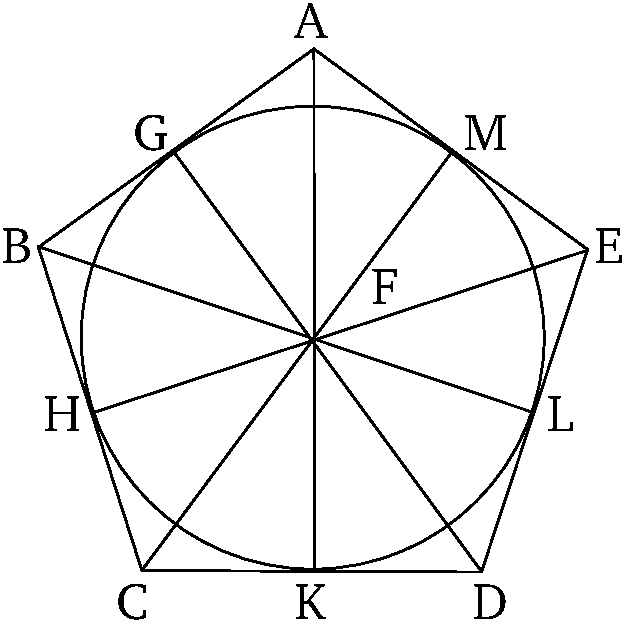
\includegraphics{Book04/fig13e.pdf}}
 
 Thus, a circle has been inscribed in the given pentagon which is
 equilateral and equiangular. (Which is) the very thing it was required to
 do.}
\end{Parallel}

%%%%%%
% Prop 4.14
%%%%%%
\pdfbookmark[1]{Proposition 4.14}{pdf4.14}
\begin{Parallel}{}{} 
\ParallelLText{
\begin{center}
{\large \ggn{14}.}
\end{center}\vspace*{-7pt}

\gr{Περὶ τὸ δοθὲν πεντάγωνον, <ό ἐστιν ἰσόπλευρόν τε καὶ 
ἰσογώνιον, κύκλον περιγράψαι.}

\gr{>'Εστω τὸ δοθὲν πεντάγωνον, <ό ἐστιν ἰσόπλευρόν τε καὶ
ἰσογώνιον, τὸ ΑΒΓΔΕ; δεῖ δὴ περὶ τὸ ΑΒΓΔΕ πεντάγωνον
κύκλον περιγράψαι.}

% Removed epsf size command
\centerline{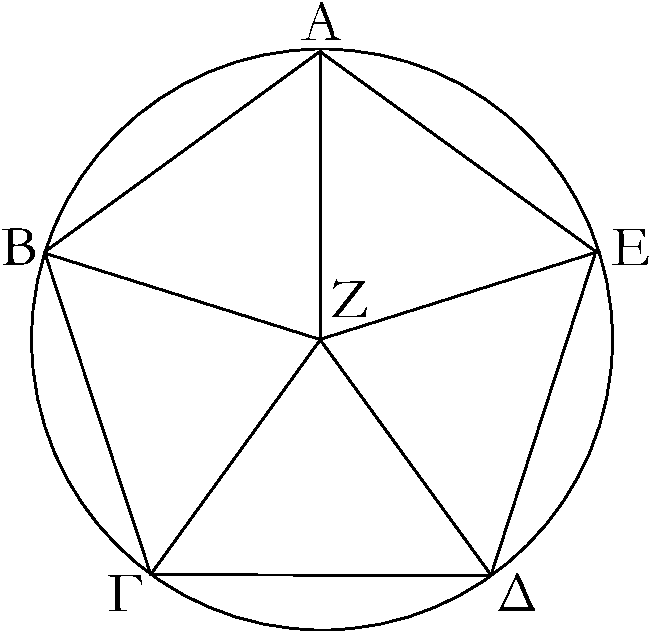
\includegraphics{Book04/fig14g.pdf}}

\gr{Τετμ\kern -.7pt  ήσθω δὴ ἑκατέρα τῶν ὑπὸ ΒΓΔ, ΓΔΕ γωνιῶν δίθα
ὑπὸ ἑκατέραξ τῶν ΓΖ, ΔΖ, καὶ ἀπὸ τοῦ Ζ σημείου,
καθ> <ὸ συμβάλλουσιν αἱ εὐθεῖαι, ἐπὶ τὰ Β, Α, Ε σημεῖα
ἐπεζεύθθωσαν εὐθεῖαι αἱ ΖΒ, ΖΑ, ΖΕ. ὁμοίωξ δὴ τῶ| πρὸ τούτου
δειθθήσεται, <ότι καὶ ἑκάστη τῶν ὑπὸ ΓΒΑ, ΒΑΕ, ΑΕΔ
γωνιῶν δίθα τέτμ\kern -.7pt  ηται ὑπὸ ἑκάστηξ τῶν ΖΒ, ΖΑ, ΖΕ
εὐθειῶν. καὶ ἐπεὶ >ίση ἐστὶν ἡ ὑπὸ ΒΓΔ γωνία τῆ|
ὑπὸ ΓΔΕ, καί ἐστι τῆξ μὲν ὑπὸ ΒΓΔ  ἡμίσεια ἡ ὑπὸ ΖΓΔ,
τῆξ δὲ ὑπὸ ΓΔΕ ἡμίσεια ἡ ὑπὸ ΓΔΖ, καὶ ἡ ὑπὸ
ΖΓΔ >άρα τῆ| ὑπὸ ΖΔΓ ἐστιν >ίση; <ώστε καὶ πλευρὰ ἡ ΖΓ
πλευρᾶ| τῆ| ΖΔ ἐστιν >ίση. ὁμοίωξ δὴ δειθθήσεται, <ότι καὶ
ἑκάστη τῶν ΖΒ, ΖΑ, ΖΕ ἑκατέρᾳ τῶν ΖΓ, ΖΔ ἐστιν >ίση; αἱ
πέντε >άρα εὐθεῖαι αἱ ΖΑ, ΖΒ, ΖΓ, ΖΔ, ΖΕ  >ίσαι ἀλλήλαιξ
εἰσίν. ὀ >άρα κέντρῳ τῶ| Ζ καὶ διαστήματι ἑνὶ τῶν ΖΑ, ΖΒ, 
ΖΓ, ΖΔ, ΖΕ κύκλοξ γραφόμενοξ <ήχει καὶ διὰ τῶν λοιπῶν
σημείων καὶ >έσται περιγεγραμμένοξ. περιγεγράφθω
καὶ >έστω ὁ ΑΒΓΔΕ.}

\gr{Περὶ >άρα τὸ δοθὲν πεντάγωνον, <ό ἐστιν ἰσόπλευρόν τε καὶ
ἰσογώνιον, κύκλοξ περιγέγραπται; <όπερ >έδει ποιῆσαι.}}

\ParallelRText{
\begin{center}
{\large Proposition 14}
\end{center}

To circumscribe a circle about a given pentagon which is equilateral and equiangular.

Let $ABCDE$ be the given pentagon  which is equilateral and equiangular.
So it is required to circumscribe a circle about the pentagon 
$ABCDE$.

% Removed epsf size command
\centerline{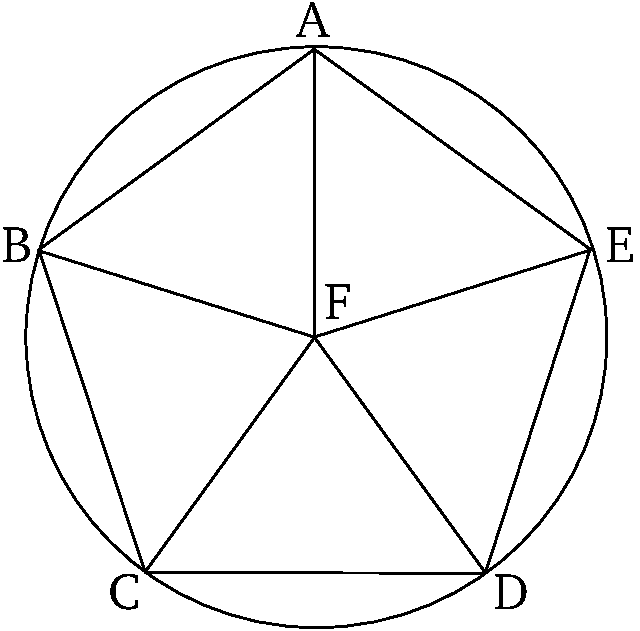
\includegraphics{Book04/fig14e.pdf}}

So let angles $BCD$ and $CDE$ have  been cut
in half by  the (straight-lines) $CF$ and $DF$, respectively [Prop.~1.9]. And let the straight-lines
$FB$, $FA$, and $FE$ be joined from point $F$, at which the
straight-lines meet, to the points $B$, $A$, and $E$ (respectively).
So, similarly, to the (proposition) before this (one), it can be shown that
angles $CBA$, $BAE$, and $AED$ have also  been cut in half by
the straight-lines $FB$, $FA$, and $FE$, respectively. And since
angle $BCD$ is equal to $CDE$, and $FCD$ is half of $BCD$, and $CDF$ half
of $CDE$, $FCD$ is thus also equal to $FDC$. So that side $FC$ is also equal to
side $FD$ [Prop.~1.6]. So, similarly, it can be
shown that $FB$, $FA$, and $FE$ are also each equal to each of $FC$ and $FD$. 
Thus, the five straight-lines $FA$, $FB$, $FC$, $FD$, and $FE$ are equal to
one another. Thus, the circle drawn with center $F$, and radius one of
$FA$, $FB$, $FC$, $FD$, or $FE$, will also go through the remaining points, and
will be circumscribed. Let it be (so) circumscribed, and let
it be $ABCDE$.

Thus, a circle has been circumscribed about the given pentagon, which
is equilateral and equiangular. (Which is) the very thing it was required to
do.}
\end{Parallel}

%%%%%%
% Prop 4.15
%%%%%%
\pdfbookmark[1]{Proposition 4.15}{pdf4.15}
\begin{Parallel}{}{} 
\ParallelLText{
\begin{center}
{\large \ggn{15}.}
\end{center}\vspace*{-7pt}

\gr{Εἰξ τὸν δοθέντα κύκλον ἑχάγωνον ἰσόπλευρόν τε καὶ ἰσογώνιον
ἐγγράψαι.}

\gr{>'Εστω ὁ δοθεὶξ κύκλοξ ὁ ΑΒΓΔΕΖ; δεῖ δὴ εἰξ τὸν ΑΒΓΔΕΖ
κύκλον ἑχάγωνον ἰσόπλευρόν τε καὶ ἰσογώνιον ἐγγράψαι.}

\gr{>'Ηθθω τοῦ ΑΒΓΔΕΖ κύκλου διάμετροξ ἡ ΑΔ, καὶ εἰλήφθω τὸ
κέντρον τοῦ κύκλου τὸ Η, καὶ κέντρῳ μὲν τῶ| Δ διαστήματι δὲ
τῶ| ΔΗ κύκλοξ γεγράφθω ὁ ΕΗΓΘ, καὶ ἐπιζευθθεῖσαι αἱ ΕΗ, ΓΗ
διήθθωσαν ἐπὶ τὰ Β, Ζ σημεῖα, καὶ ἐπεζεύθθωσαν αἱ ΑΒ, ΒΓ, ΓΔ,
ΔΕ, ΕΖ, ΖΑ; λέγω, <ότι τὸ ΑΒΓΔΕΖ ἑχάγωνον ἰσόπλευρόν τέ
ἐστι καὶ ἰσογώνιον.}\\

% Removed epsf size command
\centerline{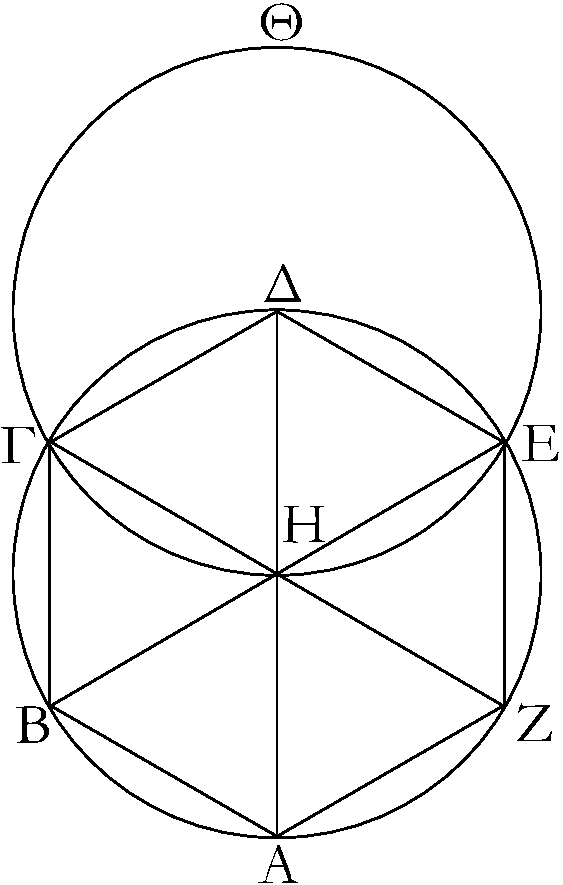
\includegraphics{Book04/fig15g.pdf}}

\gr{Ἐπεὶ γὰρ τὸ Η σημεῖον κέντρον ἐστὶ τοῦ ΑΒΓΔΕΖ κύκλου,
>ίση ἐστὶν ἡ ΗΕ τῆ| ΗΔ. πάλιν, ἐπεὶ τὸ Δ σημεῖον κέντρον
ἐστὶ τοῦ ΗΓΘ κύκλου, >ίση ἐστὶν ἡ ΔΕ τῆ| ΔΗ. ἀλλ>
ἡ ΗΕ τῆ| ΗΔ ἐδείθθη >ίση; καὶ ἡ ΗΕ >άρα τῆ| ΕΔ >ίση ἐστίν;
ἰσόπλευρον >άρα ἐστὶ τὸ ΕΗΔ τρίγωνον; καὶ αἱ τρεῖξ >άρα α\kern -.7pt  ὐτοῦ
γωνίαι αἱ ὑπὸ ΕΗΔ, ΗΔΕ, ΔΕΗ >ίσαι ἀλλήλαιξ εἰσίν,
ἐπειδήπερ τῶν ἰσοσκελῶν τριγώνων αἱ πρὸξ τῆ| βάσει γωνίαι
>ίσαι ἀλλήλαιξ εἰσίν; καί εἰσιν αἱ τρεῖξ τοῦ τριγώνου γωνίαι
δυσὶν ὀρθαῖξ >ίσαι; ἡ >άρα ὑπὸ ΕΗΔ γωνία τρίτον ἐστὶ
δύο ὀρθῶν. ὁμοίωξ δὴ δειθθήσεται καὶ ἡ ὑπὸ ΔΗΓ τρίτον
δύο ὀρθῶν.
καὶ ἐπεὶ ἡ ΓΗ εὐθεῖα ἐπὶ τὴν ΕΒ σταθεῖσα
τὰξ ἐφεχῆξ γωνίαξ τὰξ ὑπὸ ΕΗΓ, ΓΗΒ δυσὶν ὀρθαῖξ
>ίσαξ ποιεῖ, καὶ λοιπὴ >άρα ἡ ὑπὸ ΓΗΒ τρίτον ἐστὶ δύο
ὀρθῶν; αἱ >άρα ὑπὸ ΕΗΔ, ΔΗΓ, ΓΗΒ γωνίαι >ίσαι
ἀλλήλαιξ εἰσίν; <ώστε καὶ αἱ κατὰ κορυφὴν α\kern -.7pt  ὐταῖξ αἱ ὑπὸ
ΒΗΑ, ΑΗΖ, ΖΗΕ >ίσαι εἰσὶν [ταῖξ ὑπὸ ΕΗΔ, ΔΗΓ, ΓΗΒ].
αἱ <ὲχ >άρα γωνίαι αἱ ὑπὸ ΕΗΔ, ΔΗΓ, ΓΗΒ, ΒΗΑ, ΑΗΖ, ΖΗΕ
>ίσαι ἀλλήλαιξ εἰσίν. αἱ δὲ >ίσαι γωνίαι ἐπὶ >ίσων περιφερειῶν
βεβήκασιν; αἱ <ὲχ >άρα περιφέρειαι αἱ ΑΒ, ΒΓ, ΓΔ, ΔΕ, ΕΖ, ΖΑ
>ίσαι ἀλλήλαιξ εἰσίν. ὑπὸ δὲ τὰξ >ίσαξ περιφερείαξ αἱ >ίσαι
εὐθεῖαι ὑποτείνουσιν; αἱ <ὲχ >άρα εὐθεῖαι >ίσαι 
ἀλλήλαιξ εἰσίν; ἰσόπλευρον >άρα ἐστὶ το ΑΒΓΔΕΖ ἑχάγωνον.
λέγω δή, <ότι καὶ ἰσογώνιον. ἐπεὶ γὰρ >ίση ἐστὶν ἡ ΖΑ
περιφέρεια τῆ| ΕΔ περιφερείᾳ, κοινὴ προσκείσθω ἡ ΑΒΓΔ περιφέρεια; <όλη >άρα ἡ ΖΑΒΓΔ <όλῃ τῆ| ΕΔΓΒΑ  ἐστιν >ίση; καὶ βέβηκεν
ἐπὶ μὲν τῆξ ΖΑΒΓΔ περιφερείαξ ἡ ὑπὸ 
ΖΕΔ γωνία, ἐπὶ
δὲ τῆξ ΕΔΓΒΑ περιφερείαξ ἡ ὑπὸ ΑΖΕ γωνία;  >ίση 
>άρα ἡ ὑπὸ 
ΑΖΕ γωνία τῆ| ὑπὸ ΔΕΖ.  ὁμοίωξ δὴ δειθθήσεται, <ότι 
καὶ αἱ λοιπαὶ γωνίαι τοῦ ΑΒΓΔΕΖ ἑχαγώνου κατὰ μίαν 
>ίσαι εἰσὶν ἑκατέρᾳ τῶν ὑπὸ ΑΖΕ, ΖΕΔ γωνιῶν; ἰσογώνιον
>άρα ἐστὶ τὸ ΑΒΓΔΕΖ ἑχάγωνον. ἐδείθθη δὲ καὶ ἰσόπλευρον;
καὶ ἐγγέγραπται εἰξ τὸν ΑΒΓΔΕΖ κύκλον.}

\gr{Εἰξ >άρα τὸν δοθέντα κύκλον ἑχάγωνον ἰσόπλευρόν τε καὶ
ἰσογώνιον ἐγγέγραπται; <όπερ >έδει ποιῆσαι.}\\~\\~\\~\\~\\

\begin{center}
{\large \gr{Πόρισμα}.}
\end{center}\vspace*{-7pt}

\gr{Ἐκ δὴ τούτου φανερόν, <ότι ἡ τοῦ ἑχαγώνου πλευρὰ >ίση ἐστὶ
τῆ| ἐκ τοῦ κέντρου τοῦ κύκλου.}

\gr{Ὁμοίωξ δὲ τοῖξ ἐπὶ τοῦ πενταγώνου ἒαν διὰ τῶν κατὰ
τὸν κύκλον διαιρέσεων ἐφαπτομέναξ τοῦ κύκλου ἀγάγωμεν,
περιγραφήσεται περὶ τὸν κύκλον ἑχάγωνον ἰσόπλευρόν τε
καὶ ἰσογώνιον ἀκολούθωξ τοῖξ ἐπὶ τοῦ πενταγώνου
εἰρημένοιξ. καὶ >έτι διὰ τῶν ὁμοίων τοῖξ
ἐπὶ τοῦ πενταγώνου εἰρημένοιξ εἰξ τὸ δοθὲν ἑχάγωνον κύκλον
ἐγγράψομέν τε καὶ περιγράψομεν; <όπερ >έδει ποιῆσαι.}}

\ParallelRText{
\begin{center}
{\large Proposition 15}
\end{center}

To inscribe an equilateral and equiangular hexagon
in a given circle.

Let $ABCDEF$ be the given circle. So it is required to inscribe an equilateral
and equiangular hexagon in circle $ABCDEF$.

Let the diameter $AD$ of circle $ABCDEF$ be drawn,$^\dag$ and let the center $G$ of
the circle be found [Prop.~3.1].
And let the circle $EGCH$ be drawn, with center $D$, and radius
$DG$.  And $EG$ and $CG$ being joined, let them be drawn across (the
circle) to points $B$ and $F$ (respectively). 
And let $AB$, $BC$, $CD$, $DE$, $EF$, and $FA$ be joined. 
I say that the hexagon $ABCDEF$ is equilateral and equiangular.

% Removed epsf size command
\centerline{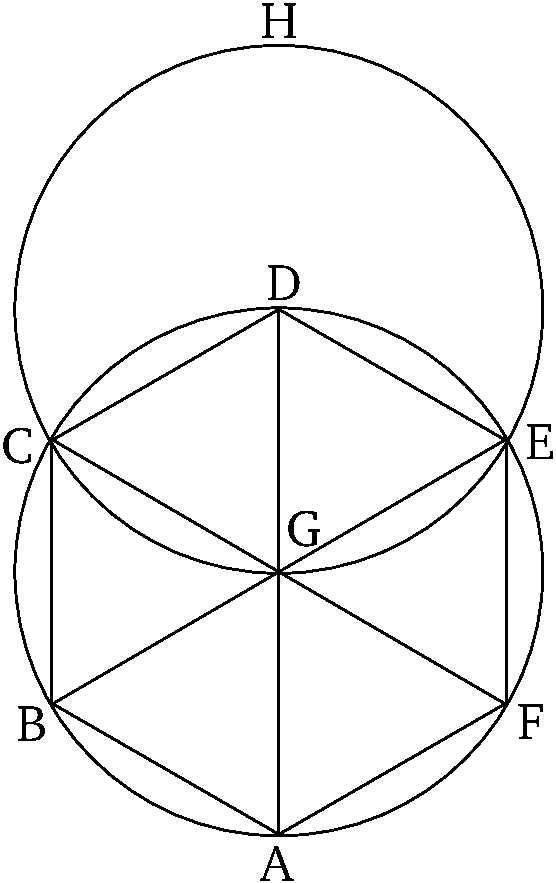
\includegraphics{Book04/fig15e.pdf}}

For since point $G$ is the center of circle $ABCDEF$, $GE$ is equal to $GD$.
Again, since point $D$ is the center of circle $GCH$, $DE$ is equal to
$DG$. But, $GE$ was shown (to be) equal to $GD$. Thus, $GE$ is also equal to
$ED$. Thus, triangle $EGD$ is equilateral. Thus, its three angles
$EGD$, $GDE$, and $DEG$ are also equal to one another, inasmuch as the angles at the base of 
 isosceles triangles are equal to one another [Prop.~1.5]. And the three angles of the
 triangle are equal to
 two right-angles [Prop.~1.32].
 Thus, angle $EGD$ is one third of two right-angles. So, similarly,
  $DGC$ can also be shown (to be) one third of two right-angles.
   And since the straight-line $CG$, standing on $EB$, makes 
 adjacent angles $EGC$ and $CGB$ equal to two right-angles [Prop.~1.13], the remaining angle
 $CGB$ is thus also one third of two right-angles.
 Thus, angles $EGD$, $DGC$, and $CGB$ are equal to one another.
 And hence the (angles) opposite to them $BGA$, $AGF$, and $FGE$
 are also equal [to $EGD$, $DGC$, and $CGB$ (respectively)] [Prop.~1.15]. Thus,
 the six angles $EGD$, $DGC$, $CGB$, $BGA$, $AGF$, and $FGE$ are equal to one
 another. And equal angles stand on equal circumferences [Prop.~3.26]. Thus, the six circumferences
 $AB$, $BC$, $CD$, $DE$, $EF$, and $FA$ are equal to one another. And
  equal circumferences
  are subtended by equal straight-lines [Prop.~3.29]. Thus, the six
 straight-lines ($AB$, $BC$, $CD$, $DE$, $EF$, and $FA$) are equal to one another.
 Thus, hexagon $ABCDEF$ is equilateral. 
 So, I say that (it is) also equiangular. For since circumference $FA$
 is equal to circumference $ED$, let circumference $ABCD$ be added
 to both. Thus, the whole of $FABCD$ is equal to the whole of
 $EDCBA$. And angle $FED$ stands on circumference $FABCD$,
 and angle $AFE$ on circumference $EDCBA$. Thus, angle
 $AFE$ is equal to $DEF$ [Prop.~3.27].
 Similarly, it can also be shown that the remaining angles of hexagon
 $ABCDEF$ are individually equal to each of the angles $AFE$ and $FED$.
 Thus, hexagon $ABCDEF$ is equiangular. And it was also shown (to be)
 equilateral. And it has been inscribed in circle $ABCDE$.
 
 Thus, an equilateral and equiangular hexagon has been inscribed
 in the given circle. (Which is) the very thing it was required to do.\\
 
 \begin{center}
{\large Corollary}
\end{center}\vspace*{-7pt}

So, from this, (it is) manifest that a side of the hexagon is equal
to the radius of the circle.

And similarly to  a pentagon, if we draw  tangents to the circle through
the (sixfold) divisions of the (circumference of the) circle, an equilateral and equiangular hexagon
can be circumscribed about the circle, analogously to the aforementioned pentagon. And, further, by (means) similar to the aforementioned pentagon,
we can inscribe and circumscribe a circle in (and about) a given hexagon. 
(Which
is) the very thing it was required to do.}
\end{Parallel}
{\footnotesize \noindent$^\dag$ See the
footnote to Prop.~4.6.} 

%%%%%%
% Prop 4.16
%%%%%%
\pdfbookmark[1]{Proposition 4.16}{pdf4.16}
\begin{Parallel}{}{} 
\ParallelLText{
\begin{center}
{\large \ggn{16}.}
\end{center}\vspace*{-7pt}

\gr{Εἰξ τὸν δοθέντα κύκλον πεντεκαιδεκάγωνον ἰσόπλευρ\-όν τε καὶ
ἰσογώνιον ἐγγράψαι.}

% Removed epsf size command
\centerline{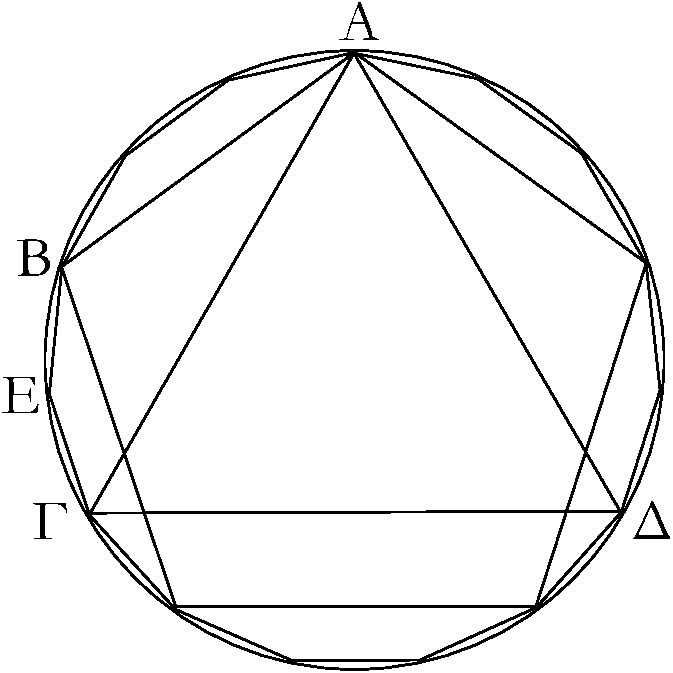
\includegraphics{Book04/fig16g.pdf}}

\gr{>'Εστω ὁ δοθεὶξ κύκλοξ ὁ ΑΒΓΔ; δεῖ δὴ εἰξ τὸν ΑΒΓΔ
κύκλον πεντεκαιδεκάγωνον ἰσόπλευρόν τε καὶ ἰσογώνιον
ἐγγράψαι.}

\gr{Ἐγγεγράφθω εἰξ τὸν ΑΒΓΔ κύκλον τριγώνου μὲν ἰσοπλεύρου
τοῦ εἰξ α\kern -.7pt  ὐτὸν ἐγγραφομένου πλευρὰ ἡ ΑΓ, πενταγώνου δὲ
ἰσοπλεύρου ἡ ΑΒ; ο<ίων >άρα ἐστὶν ὁ ΑΒΓΔ κύκλοξ >ίσων
τμ\kern -.7pt  ήματων δεκαπέντε, τοιούτων ἡ μὲν ΑΒΓ περιφέρεια τρίτον
ο>ῦσα τοῦ κύκλου >έσται πέντε, ἡ δὲ ΑΒ περιφέρεια πέμτον
ο>ῦσα τοῦ κύκλου >έσται τριῶν; λοιπὴ >άρα ἡ ΒΓ τῶν
>ίσων δύο. τετμ\kern -.5pt  ήσθω ἡ ΒΓ δίθα κατὰ τὸ Ε; ἑκατέρα >άρα τῶν
ΒΕ, ΕΓ περιφερειῶν πεντεκαιδέκατόν ἐστι τοῦ ΑΒΓΔ κύκλου.}

\gr{Ἐὰν >άρα ἐπιζεύχαντεξ τὰξ ΒΕ, ΕΓ >ίσαξ α\kern -.7pt  ὐταῖξ κατὰ 
τὸ συνεθὲξ εὐθείαξ ἐναρμόσωμεν εἰξ τὸν ΑΒΓΔ[Ε]
κύκλον, >έσται εἰξ α\kern -.7pt  ὐτὸν ἐγγεγραμμένον πεντεκαιδεκάγωνον
ἰσόπλευ\-ρόν τε καὶ ἰσογώνιον; <όπερ >έδει ποιῆσαι.}

\gr{Ὁμοίωξ δὲ τοῖξ ἐπὶ τοῦ πενταγώνου ἒαν διὰ τῶν κατὰ
τὸν κύκλον διαιρέσεων  ἐφαπτομέναξ τοῦ  κύκλου ἀγάγωμεν,
περιγραφήσεται περὶ τὸν κύκλον πεντεκαιδεκάγωνον ἰσόπλευρόν
τε καὶ ἰσογώνιον. >έτι δὲ διὰ τῶν ὁμοίων τοῖξ
ἐπὶ τοῦ πενταγώνου δείχεων καὶ εἰξ τὸ δοθὲν πεντεκαιδεκάγωνον
κύκλον ἐγγράψομέν τε καὶ περιγράψομεν; <όπερ >έδει ποιῆσαι.}}

\ParallelRText{
\begin{center}
{\large Proposition 16}
\end{center}

To inscribe an equilateral and equiangular fifteen-sided figure in a given circle.

% Removed epsf size command
\centerline{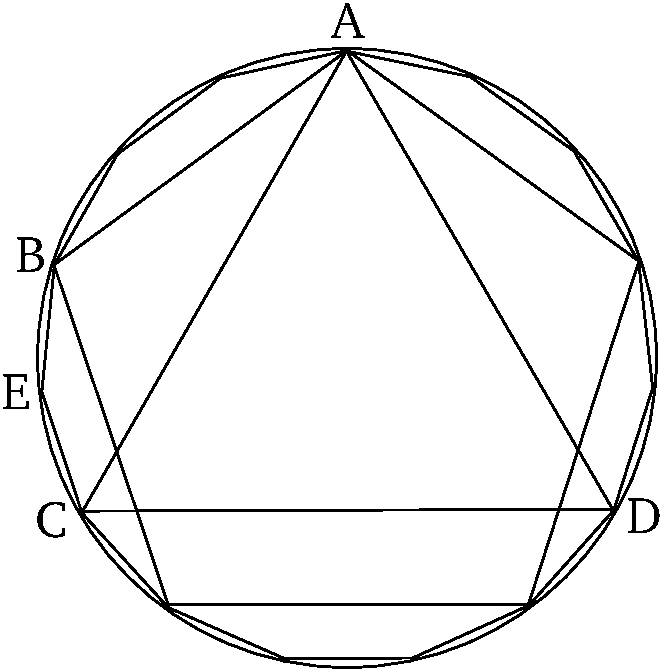
\includegraphics{Book04/fig16e.pdf}}

Let $ABCD$ be the given circle. So it is required to inscribe an equilateral
and equiangular fifteen-sided figure in circle $ABCD$.

Let the side $AC$ of an equilateral triangle inscribed in (the circle) [Prop.~4.2],
and (the side) $AB$ of an (inscribed) equilateral pentagon [Prop.~4.11],
 be inscribed in circle $ABCD$.
 Thus,   just as the circle $ABCD$ is (made up) of fifteen equal pieces, the
 circumference $ABC$, being a third of the circle, will be (made up) of five
 such (pieces), and the
 circumference $AB$, being a fifth of the circle, will be (made up) of  three.
 Thus, the remainder $BC$ (will be made up) of two equal (pieces).
 Let (circumference) $BC$ be cut in half at $E$ [Prop.~3.30].
 Thus, each of the circumferences $BE$ and $EC$ is one fifteenth of the circle
 $ABCDE$.
 
 Thus, if, joining $BE$ and $EC$, we continuously insert straight-lines
 equal to them into circle $ABCD[E]$ [Prop.~4.1],
 (then) an equilateral and equiangular fifteen-sided figure will be
 inserted into (the circle). (Which is) the very thing it was required to do.
 
 And similarly to the pentagon, if we draw  tangents to the circle through
the (fifteenfold) divisions of the (circumference of the) circle, we can
circumscribe an equilateral and equiangular fifteen-sided figure about
the circle. 
 And, further, through similar proofs to the  pentagon,
 we can also inscribe and circumscribe  a circle in (and about)  a given fifteen-sided 
  figure. (Which is) the very thing it was required to do.}
\end{Parallel}
